%todo:

%from noah 1/30 am:
%-add some more points to the x axis in figure 6 so the mosquitos prior looks bimodal. perhaps show as curves instead of bars?


% - get tiny URLs for experiment links
% - set up forest page
% - fit into space and proof read.


% - if time: look at "order effect" in prior elicitation (taboo sampling hypothesis... first sample is 0, second is 100, third - fifth are meh)
% - make figures 1 & 2 as pretty as 3 & 4




% - try rationality parameter in tfbt model
% - look at "order effect" in prior elicitation (taboo sampling hypothesis... first sample is 0, second is 100, third - fifth are meh)
% - do we really want posterior predictives that include the guessing parameter? (the guessing parameter is part of the analysis model, not the cognitive model...)
%- what kind of evidence do we want to use at the end to relate inferred priors to elicited? 
%	- is eye-balling the elicited prior and the mean inferred priors sufficient?
%	- i tried TFBT on the elicited priors to back out gamma & deltas, but gammas don't seem to come apart for DD vs. plain (as they do in the inferred priors from Exp 1 &2)
%	- one possible way to get this sort of "ordered gammas" evidence would be to repeat the prior elicitation with more items per trial
%		- the thought is that in our prior elicitation, i used 5 animals per slide (and 6 trials)
%			- probably there was not enough dynamic range for Plain vs DD to come apart 
%		- i think with 10 items, it would be better (but does that mean just 3 trials, one in each context, per subj?) [there are only 30 animals]
%% --- not sure if the above comments about prior elicitation still hold with the fixed TFBT model, but Noah's suggestion was for 1 animal at a time

%		
%todo after cogsci:
%-run additional contexts. e.g. separate dangerous and distinct.
%-look again at finer-grained truth judgement task?
%-think about the weird cases of generics in the literature. e.g. ``robins lay eggs''.
% - try an S2 model of prevalence judgement task, too. does it reduce to the L1 model?

%


% comments from workshop class 4/29
%
% why spend a lot of time in replication?
% 7 --- summary sentence 2nd paragraph to intro
% abstract worrisome
% look at study discussions -- move stuff to intro
%
% Lay eggs vs. Are female /// John is tall vs. ESB is tall [move even earlier]
% Move "a natural foil" earlier
%
% Maybe add talk of stereotypes?
% Craig: Use speaker / listener actors more; think about the person and the thing they're doing
% 
% Simulations of theoretical analysis: first sentence WHOA
%
%  beef up penultimate paragraph in intro: talk about why distinctive and dangerous are important
% ---- unpack distinctive and dangerous (use experimental materials)
%
% TABLE for materials and experiment. 
% maybe set up replication-idea early.  and then go on.




% details
%
% Section 4: exp 2 intro
%% oceans underneath each sentence
%% connect back with behavior--- asymmetry, truth cond
%
% pre Exp 3: use 
% "endemic to the entire category"
% exp3a: jargon word 
% (reuse penultimate intro paragraph throughout) [maybe make higher level version of this paragraph for intro]
%
% pre-experiments, "Like Exp 2c, 3b did BLAH but differed "
%
% add more to figure captions?
%
%
% seeds of very last paragraph in earlier
%
% in conclusion: what do the tools allow us to do? (e.g. w/ stereotyping) 
% differences in prior knowledge --> how does this contribute to language change?
% 




\documentclass[10pt,letterpaper]{article}
% Default margins are too wide all the way around. I reset them here
%\setlength{\topmargin}{-.5in} \setlength{\textheight}{9in}
%\setlength{\oddsidemargin}{.125in} \setlength{\textwidth}{6in}

\usepackage{setspace}
\doublespacing

\usepackage{geometry}
\geometry{legalpaper, margin=1in}

\usepackage{pslatex}
\usepackage{apacite}
\usepackage{url}
\usepackage{graphicx}
\usepackage{caption}
\usepackage{subcaption}
\usepackage{listings}
\usepackage{color}
\usepackage{textcomp}
\usepackage{amsmath}
\usepackage{amssymb}
\usepackage{wrapfig}
\usepackage{lipsum}

\graphicspath{{figures/cogsci/}}

\def\signed #1{{\leavevmode\unskip\nobreak\hfil\penalty50\hskip2em
  \hbox{}\nobreak\hfil(#1)%
  \parfillskip=0pt \finalhyphendemerits=0 \endgraf}}

\newsavebox\mybox
\newenvironment{aquote}[1]
  {\savebox\mybox{#1}\begin{quote}}
  {\signed{\usebox\mybox}\end{quote}}


 \newcommand{\denote}[1]{\mbox{ $[\![ #1 ]\!]$}}


%\lstset{
%  language=Scheme, % Andreas Stuhlmuller. Scheme listings. https://github.com/stuhlmueller/scheme-listings.git
%  columns=fixed,
%  tabsize=2,
%  extendedchars=true,
%  breaklines=true,
%  frame=single,
%%  numbers=left,
%  numbersep=5pt,
%   basicstyle=\scriptsize\ttfamily
%%  rulesepcolor=\color{solarized@base03},
%%  numberstyle=\tiny\color{solarized@base01},
%%  keywordstyle=\color{solarized@green},
%%  stringstyle=\color{solarized@cyan}\ttfamily,
%%  identifierstyle=\color{blue},
%%  commentstyle=\color{solarized@base01},
%%  emphstyle=\color{solarized@red}
%}

\definecolor{Red}{RGB}{255,0,0}
\newcommand{\red}[1]{\textcolor{Red}{#1}}  

\title{Words are vague: A prevalence-based account of generic language}
% \title{Generic statements are vague}
% \author{{\large \bf Michael Henry Tessler, Noah D. Goodman } \\
%	\{mhtessler, ngoodman\}@stanford.edu \\
%  Department of Psychology, Stanford University}

\author{{\large \bf Michael Henry Tessler} (mtessler@stanford.edu)\\ {\large \bf Noah D. Goodman} (ngoodman@stanford.edu) \\
  Department of Psychology, Stanford University}
 
\begin{document}
%\newpage
%\tableofcontents
%\newpage
%\listoffigures
%\newpage
\maketitle


\begin{abstract}
Generic utterances (e.g. ``Dogs bark'') are ubiquitous in natural language. Despite their prevalence, the meanings of generic statements are puzzling to formal approaches. For example, what percentage of the category must display the property (i.e. what threshold must the prevalence cross) for the generic to be true? Here, we formalize a prevalence-based semantics, wherein the threshold for acceptance is represented as an unknown property of the language by the listener, and must be actively reasoned about in context by the listener. To illustrate the model, we measure participant's prior expectations about the prevalence of certain properties of theoretical interest. We show how point-wise prevalence cannot account for truth values the associated generic statements, and how a more elaborate account based on distributions of prevalence and conversational principles can. Generic statements are additionally puzzling because they can be accepted for a range of prevalence levels but are often interpreted as applying to nearly-all of the category. We replicate a controlled experimental finding validating this intuition and show how the prevalence-based model predicts this asymmetry between truth value judgments and interpretations. This work suggests that the semantics of generic statements can treated as scalar, and that generic statements are foremost statements about the prevalence of properties.

%We illustrate the model by showing its ability to capture gender-specific and low-prevalence generics---two cases of theoretical importance
%We replicate two major previous findings: (1) Generics about dangerous or distinctive properties are more acceptable than similar generic statements such connotations, and (2) Novel generic statements (e.g. ``Lorches have purple feathers) are interpreted as applying to nearly all of a category (i.e. almost all lorches have purple feathers) while the same statements are accepted as true for a wide range of prevalence levels (e.g. when only 10\% of lorches have purple feathers). The prevalence-based model predicts (1) [differential acceptability of generics] if the prior distribution over the prevalence (i.e. the probability of the property given the category) differs between these different types of properties. The prevalence model also predicts (2) [strong implications of generic] if the prior over prevalence is bimodal with a peak at 100\%. We find direct evidence that this is so by eliciting the prior distribution over prevalence empirically. 
%
%
%Here, I formalize a prevalence-based
%semantics, wherein the threshold for acceptance is represented as an unknown
%property of the language, and must be actively reasoned about in context by the
%listener. I will illustrate this model by showing its ability to capture gender-specific
%and low-prevalence generics---two cases of theoretical importance. I?ll go on to show
%how this model can account for previous empirical findings that (1) Generics about
%dangerous and distinctive properties are more acceptable than similar generic
%statements lacking such connotations, and (2) Novel generic statements (e.g.
%?Lorches have purple feathers?) are interpreted as applying to nearly all of a
%category (i.e. almost all lorches have purple feathers) while the same statements are
%accepted as true for a wide range of prevalence levels (e.g. when only 30% of
%lorches have purple feathers). I?ll try to conclude by discussing future directions of
%this work relating to the pragmatics of experimental contexts.


%demonstrated that the endorsement rate of generic statements differs by context, and that generics can be endorsed based on weak evidence while the same sentences are interpreted strongly. Here, we replicate these effects in Exp.~1 and investigate how models based on prevalence (the probability of the property given the category) can account for this behavior. 
%Using Bayesian data analysis techniques, %to make inferences about the putative threshold used as well as to arbitrate between competing accounts. 
%we show how a simple scalar prevalence semantics is untenable, but that the same semantics within a probabilistic pragmatics framework can account for the data. 
%In this model, the generic has an underspecified meaning, but this uncertainty is resolved by context and interaction. 
%Context effects are predicted if the prior distribution of prevalence differs by context; in Exp.~2 we find direct evidence that this is so.
%The differences between verification and interpretation are understood as different tasks within a communicative framework. 
%We use a Bayesian analysis again to infer a prior distribution, for which we then find confirmatory evidence in Exp. 2. 


\textbf{Keywords:} 
generics; pragmatics; bayesian model
\end{abstract}

%\begin{aquote}{John Locke, \emph{An Essay Concerning Human Understanding (1690)}}
%Now since [articulate] sounds have no natural connexion with our ideas, but have all their signification from the arbitrary imposition of men, the doubtfulness and uncertainty of their signification has its cause more in the ideas they stand for than in any incapacity there is in one sound more than in another to signify any idea: For in that regard they are all equally perfect.
%\end{aquote}


Imagine talking with a 3-year-old about oxygen. Oxygen is difficult to explain because it is so rarely observable and the function of oxygen is abstract. You might offer, ``Animals breathe oxygen to live.''. Few would argue with the truth of this sentence, yet its meaning is difficult to specify. 

%Is it synonymous with ``All animals breathe Oxygen to live''? %It's false that \emph{all} animals breathe oxygen (e.g. fish), yet intuitively the sentence seems to convey something stronger than the weak \emph{some} animals breathe oxygen. 
%If you were talking with an adult, you might use a more nuanced statement (e.g. by talking about the subcategory Mammals).
%Words are vague because ideas are vague, Locke argues. In making this argument, he falls into the habit of communication that we all fall into: using generalizations about members of a category---in this case, \emph{[articulate] sounds}. 
%

This type of utterance is generic \cite{Carlson1977, Leslie2008} in that it conveys a generalization about a category. At first glance, generics statements might seem to mean the same as universally-quantified statements (i.e. ``All animals breathe oxygen''). Unlike ``all''-statements, however, generics are resilient to counter-examples: ``Animals breathe Oxygen to live'' is true even though there are three species of creatures called \emph{lorica} that live 2.2 miles underwater on the ocean floor in an oxygen-free environment \cite{Danovaro2010}. You might think, then, that generics are synonymous with weaker ``most''-statements. However, we'll only be able to maintain this logic until we encounter generics like ``Birds lay eggs'' or ``Mosquitos carry West Nile Virus'', which are both intuitively true despite the fact that only adult female birds lay eggs and that less than 1\% of mosquitos carry West Nile Virus. The only quantifier that could satisfy all of these conditions is the existential ``some''.  Yet, the semantics for ``some'' cannot be the semantics of generics:  Upon hearing a generic, listeners are wont to interpret the sentence as applying to \emph{all or nearly all} of a category \cite{Gelman2002, Cimpian2010}. ``Some animals breathe oxygen'' implies something quite different (e.g. that not all animals breathe oxygen) \cite{Degen2015}.


% Generics can be true based on very little evidence (e.g. each of us has encountered only a small number of all the animal-kinds in the world). % should I deply the mosquitos here?
%
%is making his argument not based on a corpus study of words but based on his intuition and the particular examples he is considering implicitly, a relatively small proportion of the potential infinitude of articulate sounds. 
%
%At the same time, generics are robust to counterexamples
%
%Locke's argument is still tenable even if we know that we know there are non arbitrary word--meaning mappings (hence, ``\emph{all} sounds have no natural connexion with our ideas'' is false, \red{cite bouba-kiki, erin?, molly?}). 
%
%Finally, generics have strong implications.%

What could be the stable meaning of a generic given this extreme flexibility? We propose these phenomena can be explained as the effects of pragmatic inference filling in a meaning that is underspecified in the language. 
%
 %We propose that the meaning of a generic is underspecified in the language and these phenomena can be explained as the effects of pragmatic inference over this underspecified meaning. %
 %
In particular, we posit that generics are vague in the way that gradable adjectives like \emph{tall} are vague. To understand the vagueness of ``tall'', consider the conditions under which a person would qualify as ``tall'' versus the conditions for a building to qualify as ``tall''.
The vagueness and context-sensitivity can be accounted for by treating $\theta_{tall}$ as an unknown property of the language, and modeling the listener as inferring this threshold in context \cite{Lassiter2015}. In this example, different thresholds are derived through the interaction of the prior distribution over heights (people vs. buildings) with the communicative pressures to be truthful and informative. 
 
%In a similar way, we posit a simple, scalar semantics for generics in which they express that the probability of the property given the kind-----i.e. the property's \emph{prevalence}-----is above a threshold (cf. \citeA{Cohen1999}). Following \citeA{GoodmanLassiter}, we treat this threshold as unknown property of the language and thus, as a variable that must be reasoned about in context. In this way, generics are vague in the way gradable adjectives like ``tall'' are vague: There is inherent uncertainty in the words' context-independent meaning. In this extension of the \emph{Rational Speech-Act} (RSA) framework \cite{Frank2012,Goodman2013}, the listener is tasked with the joint problem of figuring out what the speaker intended to communicate as well as what the generic means \emph{in this context}. 

In a similar way, we posit a simple, scalar semantics for generics in which they express that the probability of the property given the kind-----i.e. the property's \emph{prevalence}-----is above a threshold (cf. \citeA{Cohen1999}). We treat this threshold as unknown property of the language and thus, as a variable that must be reasoned about in context. In this extension of the \emph{Rational Speech-Act} (RSA) framework \cite{Frank2012,Goodman2013}, the listener is tasked with the joint problem of figuring out what the speaker intended to communicate as well as what the generic means \emph{in this context}. 

With uncertainty in the language, the listener figures out what the words mean by drawing upon her prior beliefs---in this case about the prevalence of the property---in addition to harnessing standard inferences from conversational pragmatics \cite{Clark1996, Grice1975, Levinson2000}. From this, this model predicts the degree to which a given generic utterance will be acceptable, and predicts how this might vary for different types of properties. At the same time, the model predicts that a generic utterance will have variable interpretations contingent on the prior distribution on prevalence. We explore these predictions in this paper.
%
\subsection{The phenomena}

One important test for a theory of generic meaning is that it captures the intuition shared by philosophers, linguists, and psychologists about the truth of certain example sentences. To test the predictions of this model, we must first measure participant's prior expectations about the prevalence of the properties in question. Critically, however, we must measure not only prior expectations about the prevalence of the property for the category but the distribution of expectations across categories (i.e. not only the probability of laying eggs for a bird, but also the probability of laying eggs for a cow and other animal species).  We show how point-wise prevalence is insufficient to explain generic acceptability, but a model that considers the distribution over prevalence is sufficient to explain the variability in truth judgments for generics.

Generic statements not only vary in acceptability, but also in how they are interpreted. \citeA{Cimpian2010} used a pair of tasks to assess the relationship between the \emph{truth judgments} and \emph{interpretations} of novel generic statements. In these studies, the \emph{interpretations} of generic statements were measured by asking participants to report the prevalence of the property within the category upon hearing the associated generic, e.g. ``Lorches have purple feathers. What \% of lorches do you think have purple feathers?'' In this task, subjects reported that almost all of the category had the property (i.e. almost all lorches have purple feathers.). In the \emph{truth judgments} task, participants were given prevalence information (e.g. ``30\% of lorches have purple feathers.'') and asked if the associated generic statement (i.e. ``Lorches have purple feathers'') was true or false. The results suggest an apparent ``paradox'' in the form of an asymmetry between the truth judgments of generics and the interpretations of generics:  Generics are accepted at prevalence levels as low as 10\%, but are interpreted as applying to nearly 100\% of the category\footnote{This asymmetry was absent for the sentences that used the quantifier ``most'', arguably the quantifier with the most similar meaning to generics \red{[cite]}}.  In a follow-up experiment, the authors showed how the interpretations of generics can be greatly weakened if the property in question is not a biological property (e.g. ``purple feathers'') but instead an accidental property (e.g. ``muddy feathers''). We replicate these findings and show how the apparent ``paradox'' can be explained by the interaction of an uncertain semantics with a prior distribution over the prevalence of biological properties. We further show how the interpretations of generics can be substantially weakened when the listener considers the distribution of prevalence for accidental properties.

%
%We demonstrate that the model captures cases of theoretical importance: gender-specific and low-prevalence generics. We replicate the main effects reported by \citeA{Cimpian2010} and use Bayesian data analytic techniques to further examine how the effective truth conditions of generic statements interact with the prior on prevalence. We show that our model predicts both flexible truth conditions and asymmetry effects, given appropriate priors over prevalence (``\emph{backward predictions} of the model''). We experimentally elicit the prevalence priors in CBG's experimental contexts, verifying these predictions (Expt.~2). We show that the elicited prevalence priors predict the same effects as the inferred priors (``\emph{forward predictions} of the model''), and then show how the effects dissipate when different types of properties (with different types of priors) are discussed (Expt.~3). Finally, we explore a case when the flexibility of truth conditions are difficult to associate with prevalence (Expt.~4). 


%\subsection{Previous findings}
%Determining the truth of individual generic statements is typically left to the intuitions of linguists \cite{Carlson1977, Leslie2008}. Psychological investigations have provided a complementary avenue to understanding the meaning of generic language by controlling for	various intrinsic differences between the examples considered by linguists. \citeA{Cimpian2010} carried out a series of experiments designed to examine the acceptability and implications of generic statements about novel animal categories (e.g.~``Lorches have purple feathers'') . 
%They found evidence that if the property in question was dangerous (e.g. ``These feathers are as sharp as needles and can easily get lodged in you, causing massive bleedings.'') or distinctive (e.g. ``No other animals have these kinds of feathers.''), the associated generic (i.e. ``Lorches have purple feathers'') was endorsed more and at lower prevalence levels (e.g. when only 10\% of lorches had purple feathers). This finding suggests that the conditions under which a generic is true---the generic's \emph{truth conditions}---vary as a function of the type of property being discussed (e.g. a dangerous property, a distinctive property). Distinctive properties are theoretically interesting because they intuitively map onto naturally-occurring generic statements that participant's readily endorse (e.g. ``Birds lay eggs'', ``Cardinals have red feathers''). In a similar vein, dangerous properties are intriguing because the truth conditions of such generic statements seem to be divorced from the prevalence of the property as in ``Mosquitos carry West Nile Virus'' ($<$ 1\% of mosquitos carry the virus) and ``Sharks attack swimmers''.
%
%\citeA{Cimpian2010} used a complementary task to assess the \emph{implications} of generic statements. In these studies, the \emph{implications} of generic statements were measured by asking subjects prevalence questions, e.g. ``What \% of lorches do you think have purple feathers?'' In this task, subjects reported that almost all of the category had the property (i.e. almost 100\% of lorches have purple feathers.). This raises an apparent asymmetry between the truth conditions of generics (generics are accepted at prevalence levels as low as 10\%) and the implications of generics (generics are interpreted as applying to nearly 100\% of the category). 

%\subsection{The current investigations}


%The asymmetry effects fall out of modeling task differences between the language understanding and answer-selection tasks faced by participants in the different experiments (cf. \citeA{Degen2014}). 
%Presumably, Locke is arguing about \emph{almost} all words. Why else would he go through the trouble of crafting this argument?
%
%\red{
%In this paper, we will see that the \emph{context} in which his words are uttered is essential to the meaning we derive. We propose that this aspect of generic language follows from pragmatic reasoning about an uncertain threshold for meaning; an idea which we formalize in a probabilistic model within the Rational Speech Acts framework \cite{Frank2012,Goodman2013}.
%%
%Generic statements are puzzling because their meaning is so flexible. On the one hand, generics would seem to suggest an almost universal quantification, as in ``Dogs bark''. Others, like ``Mosquitos carry West Nile virus'', involve a property that applies only to a small subset of the kind. 
%}
%It is perhaps this inherent uncertainty that leads generics to be so widespread in natural language. 


 %suggested that different dependent measures in experimental pragmatics paradigms map onto different communicative roles, and thus should be modeled accordingly. 

%We draw on new advances in probabilistic pragmatics to formalize two possible theories of the generic. Further, we harness the power of Bayesian data analysis to mediate between these formal theories and draw inferences about cognitively interesting model parameters. 


%(e.g. ``These feathers are as sharp as needles and can easily get lodged in you, causing massive bleeding. No other animals have these kinds of feathers'')
% (e.g.  ``These feathers are wide and very smooth to the touch. Other animals have these kinds of feathers.'')

%How are we to understand these data? One interpretation is that context changes the truth-conditions for a generic statement, but that within a context, the truth-conditions are stable. A different sort of explanation is that context changes the nature of world somehow, and that generic meanings are inferred rationally from context. We draw on recent advances in probabilistic pragmatics and Bayesian data analysis to mediate between these two alternatives.

\section{A lifted-threshold model of generic meaning}

We view language understanding as a special case of social cognition, and language comprehension as deriving from an intuitive theory of language production.  We draw on recent work from probabilistic pragmatics to formalize how listeners arrive at interpretations of generic utterances. In particular, we draw on work from the Rational Speech-Act (RSA) theory of language understanding. In this framework, a listener infers the meaning of an utterance by considering the thought-processes of a speaker whose goal is to be informative. Variants of this theory have provided formal explanations for a number of linguistic phenomena including scalar implicature, hyperbole, and argument evaluation \cite{Kao2014, Tessler2014, Lassiter2014}. 

%CBG showed how contexts affects the endorsement for generic statements. An additional concern of their experiments surrounded the relation between two dependent measures for understanding generics. One dependent measure was the ``truth conditions'', or \emph{sentence verification} measure that we've been considering up to this point. The other was an ``implied prevalence'', or \emph{sentence interpretation} dependent measure. The latter was collected by giving participants the generic statement (plus, any additional contextual information), and asking the participant ``What percentage of lorches have purple feathers?''

%The tasks in Exp.~1 are, fundamentally, language understanding tasks. Participants are given premises and asked to draw a conclusion that necessarily involves reasoning about the meaning of words. 

%\subsection{Lifted-variable RSA}

%The Bayesian data analysis above provides compelling evidence that context influences the truth-conditions of a generic statement. The poor qualitative fit as well as the high inferred value of the guessing parameter $\phi$ suggest, however, that our language model is incomplete. Rather than propose that the meaning of a generic is simply a one-to-one mapping between context and threshold, 


We propose that generics are vague. In this way, generics are similar to gradable adjectives like \emph{tall}. 
%% 
%\red{MOVE THIS EARLIER}
%For example, the conditions under which ``John is tall'' and ``The Empire State Building is tall'' are quite different. 
%\red{++++}
%
\citeA{Lassiter2015}  propose the meaning of an adjective like \emph{tall} is a standard truth-functional, threshold meaning such that the object in question \emph{is tall} if it has a height greater than the threshold $\theta_{tall}$. 
%
%The vagueness and context-sensitivity of these adjectives are accounted for by treating $\theta_{tall}$ as an unknown property of the language, and modeling the pragmatic listener as inferring this threshold. In this example, different thresholds are derived through the interaction of the prior distribution over heights (people vs. buildings) with the communicative pressures to be truthful and informative. 
 %
In a similar way, we propose the literal semantics of a generic sentence is in fact a threshold on prevalence, but listeners have uncertainty about the threshold \emph{a priori} and actively must reason about it in context. The relevant prior distribution is the distribution of the property across categories (e.g. 0\% of lions lay eggs, 50\% of birds lay eggs, ...). Just as the prior distributions of heights for people and buildings differ, the prior distributions of prevalence for different types of properties can vary.

The RSA model for generic interpretation, with the prevalence threshold as a variable ``lifted'' to pragmatic reasoning is specified by:
\begin{flalign}
& P_{L_{1}}(x , \theta \mid g) \propto P_{S_{1}}(g \mid x, \theta) P(x) \label{eq:L1}
\end{flalign}
Eq.~\ref{eq:L1} is a model of a listener ($L_{1}$) who has been told a generic statement $g$. She has uncertainty about the prevalence of the property $x$ as well as the meaning of the generic $\theta$, and is trying to figure out what these are. She accomplishes this by assuming that this generic was produced by a speaker $S_{1}$, whose goal was to communicate the prevalence of the property $x$. The speaker model is specified by:
\begin{flalign}
& P_{S_{1}}(g \mid x, \theta) \propto \exp(\lambda \ln {P_{L_{0}}(x \mid g, \theta)}) \label{eq:S1}
\end{flalign}
This is a model of a speaker who knows some prevalence $x$ to be the case (e.g. knows that 50\% of birds lay eggs). The listener ($L_{1}$) believes that the speaker ($S_{1}$) has a particular threshold $\theta$ in mind: Hence, the listener has uncertainty about what the words mean, but assumes that the speaker --- who produced those words --- know what they mean. The listener's intuitive theory of speaker also assumes the speaker chooses his words to be informative to a hypothetical literal listener, specified by:

\begin{flalign}
& P_{L_{0}}(x \mid g, \theta) \propto {\delta_{\denote{g(\theta)}(x)} P(x)} \label{eq:L0}
\end{flalign}
Here $\denote{g(\theta)}: X \rightarrow \text{Boolean}$ is a truth-function specifying the literal meaning of the generic. The literal content in Eq.~\ref{eq:L0} is given by $\denote{g(\theta)}= \{x | x > \theta \}$, where $x$ is a prevalence. $g$ is a function of $\theta$ because the meaning of a generic may vary across contexts.

The degree to which the speaker's utterance is optimal for a given intended-prevalence is governed by a soft-max decision rule with rationality parameter  $\lambda$ \cite{Luce1959}. From this, the pragmatic listener (Eq. ~\ref{eq:L1}) jointly infers both the prevalence $x$ and the threshold $\theta$. We call this type of model a ``lifted threshold'' model because $\theta$, traditionally thought to be part of the semantic content of the utterance (and thus perfectly transparent to all in the conversation), has been underspecified in the semantics but is locally fixed through pragmatic reasoning.
 
%However, it interacts with the prior distribution $P(x)$ over prevalence levels---the prior distribution across kinds of a particular property's prevalence.

%The prevalence prior $P(x)$ has a critical effect on the interpretation of the generic in this model. Since $\theta$ is actively reasoned about, it will be set to values that balance truthfulness and informativity. Consider two generic statements: ``Humans breathe oxygen'' and ``Humans breathe polluted air''. Figure \ref{fig:ex}
%
%\begin{figure}
%\centering
%    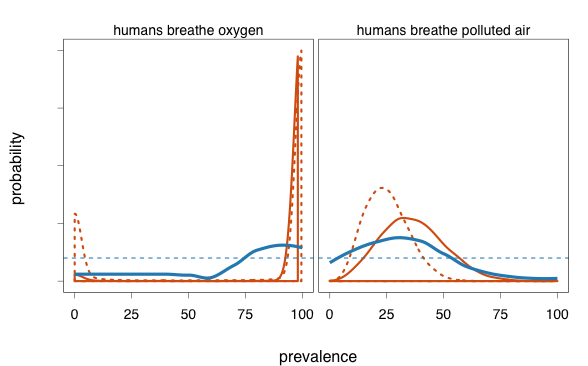
\includegraphics[width=0.7\columnwidth]{example}
%    \caption{Different priors on prevalence lead to dramatically different interpretations of the generic. Orange: prevalence. Blue: threshold for the generic to be true. Dotted lines denote priors and solid lines denote posteriors. Breathing oxygen is something that almost every animal-kind does (and within each kind, 100\% of them do). Breathing polluted air is a more accidental condition, and animal kinds will differ in how many of them are exposed to polluted air.}
%  \label{fig:ex}
%\end{figure}
%
%
%Consider again the case of vague adjectives. \emph{Tall} means something different if it is predicating ``John'' than if it is predicating ``The Empire State Building'' because the distributions over heights vary for people and buildings. In the people domain, $\theta_{tall}$ will probably be set somewhere around 6 feet, since this is above the mean (and hence, would be informative) but not too far above the mean (hence, would still be truthful). 

%\subsection{The \emph{Question Under Discussion}}
%
%To connect this model to the dependent measures used in the experiments that follow, we introduce another level to the model. One of the tasks is a true-false judgment task, which we model as a speaker who can either say ``[[the generic]] is true'' or ``[[the generic]] is false''.
%
%\begin{equation} 
%P_{S_{2}}(g \mid x) \propto {P_{L_{1}}(x \mid g)}.
%\label{eq:S2}
%\end{equation}
%
%This speaker in \eqref{eq:S2}, like $L_{1}$, doesn't know the threshold, but knows that $L_{1}$ is thinking about it, and marginalizes over possible values: $ P_{L_{1}}(x \mid g) = \sum_{\theta} P_{L_{1}}(x , \theta \mid g) $.
%
%In the other task, participants are given a generic utterance and asked to judge the prevalence of the property. 
%



%As a first test the model, we posit a family of possible priors $x \thicksim \beta(\gamma,\delta)$\footnote{For ease of interpretation, we are parametrizing the $\beta$ distribution by its mean and concentration. To recover the canonical shape parametrization, use $\gamma \delta$ and $(1-\gamma)\delta$.}. We hypothesize that the details of these priors (i.e.~$\gamma$'s and $\delta$'s) may differ according to the type of property in reference by the generic. For instance, when you know that a particular property is rare, a different distribution of that property over kinds is called to mind, than if the property is common. This would result in different meanings for the generic. Below we infer appropriate prior parameters for each property-type from the behavioral data.
%
%Following the advice of \citeA{Degen2014}, who investigated the relationship between dependent measures and speaker and listener roles in RSA, we will model the \emph{implied prevalence} task as a pragmatic listener ($L_{1}$) task, but the \emph{truth conditions} task as a pragmatic speaker task. We model the truth judgment with a speaker $S_{2}$ who is trying to convey the prevalence to a pragmatic listener, but can only produce the generic or its negation (i.e.~yes or no to the truth of the generic):

\subsection{Simulations of theoretical interest}
\label{sec:simulations}

We propose that a model of generics with a scalar semantics on prevalence is tenable if the threshold is left underspecified in the semantics. This section explores the influence of different prevalence priors on different truth conditions for a few examples of theoretical interest. To connect our model of generic interpretation to generic truth conditions, we include an additional component to the model: a speaker who can either say ``[[the generic]] is true'' or ``[[the generic]] is false'' \cite{Degen2014}:

\begin{equation} 
P_{S_{2}}(g \mid x) \propto \exp(\lambda \ln {P_{L_{1}}(x \mid g)}).
\label{eq:S2}
\end{equation}


This speaker in \eqref{eq:S2}, like $L_{1}$, doesn't know the threshold, but knows that $L_{1}$ is thinking about it, and marginalizes over possible values: $ P_{L_{1}}(x \mid g) = \sum_{\theta} P_{L_{1}}(x , \theta \mid g) $. The $S_{2}$ speaker has in mind a prevalence $x$ (or, equivalently here, a category--property pair corresponding to that prevalence), e.g. ``birds'' and those that ``lay eggs''. The speaker then reasons whether it would be better to say ```Birds lay eggs' is true''  or ```Birds lay eggs' is false'' in order to convey the state of the world, namely that about 50\% of birds lay eggs\footnote{Technically, the prevalence of birds laying eggs is closer to 35\%, as only \emph{adult}, female birds lay eggs. We gloss over this detail here.}. The speaker selects the utterance according to a soft-max decision rule governed by parameter $\lambda$\footnote{It's conceivable that this $\lambda$ is different from the parameter that governs the selection of $S_{1}$'s utterances. For simplicity here we assume they are the same.}.

Continuing with this example, the speaker imagines the likely prevalence that the pragmatic listener $L_{1}$ will infer given either ```Birds lay eggs' is true''  or ```Birds lay eggs' is false''. Here, the prevalence prior plays a critical role in determining where the generic-threshold $\theta$ (and, consequently, the resulting inferred prevalence $x$) is likely to fall (Figure \ref{fig:schematic}). In setting the threshold, the pragmatic listener $L_{1}$ balances the truth of the utterance with the informativeness of the utterance. If ```Birds lay eggs' is true'', the pragmatic listener $L_{1}$ will likely set the threshold $\theta$ below 50\%, as this is necessary to make the utterance true (Figure \ref{fig:schematic}; red). At the same time, $L_{1}$ believes the message to be informative, so she will set $\theta$ probably above 10\%. Since the prevalence has to be above the threshold in order to make the utterance true, the most likely inferred prevalence $x$ will be about 50\% (i.e. after ruling out everything below 10\%, the most probably prevalence will be 50\%). On the other hand, if the speaker were to say ```Birds lay eggs' is false'', the prevalence would have to fall \emph{below} the threshold, which in this case would implicate the mass below 10\% and the pragmatic listener would infer something the speaker didn't intend. 

\begin{figure}[t]
  \begin{center}
    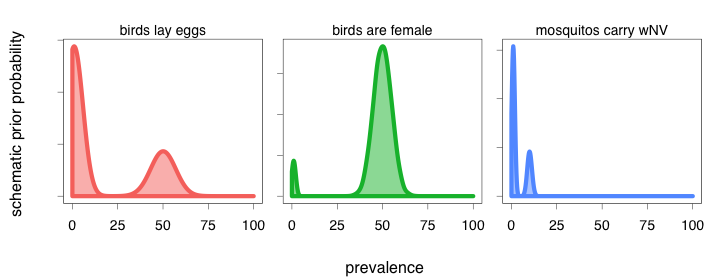
\includegraphics[width=0.8\columnwidth]{schematicPriors}
  \end{center}
  \caption{Schematic priors over prevalence for generics like ``Birds lay eggs'', ``Birds are female'', and ``Mosquitos carry West Nile Virus''.}
   \label{fig:schematic}
\end{figure}

A natural foil for this example is ``Birds are female''. For birds, ``lay eggs'' seems to have the same prevalence as ``are female'' but many speakers judge the generic ``Birds are female'' to be false \cite{Khemlani2009, Brandone2012}.  ``Birds are female'' is different from ``Birds lay eggs'' because the overwhelming majority of animal kinds are about 50\% female (see Figure \ref{fig:schematic}; green). By contrast, very few animal kinds have any egg layers; those animal kinds that do have about 50\% egg layers (Figure \ref{fig:schematic}; red). The lifted threshold RSA model is ambivalent between the saying ```Birds are female' is true'' and ```Birds are female' is false'', while at the same time, has a clear preference for supporting ``Birds lay eggs'' (Figure \ref{fig:schem_tc}; medium prevalence, red vs. green bars).

\begin{figure}
  \begin{center}
    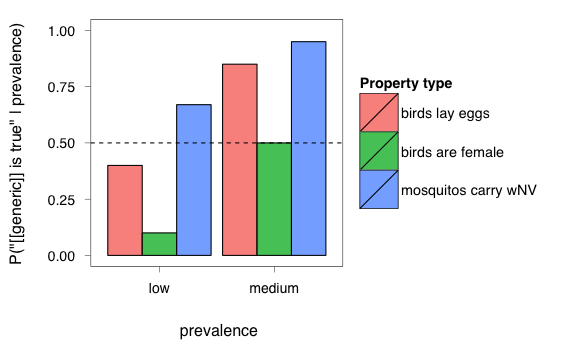
\includegraphics[width=0.8\columnwidth]{schematic_tc_bars}
  \end{center}
  \caption{Schematic truth conditions for generics like ``Birds lay eggs'', ``Birds are female'', and ``Mosquitos carry West Nile Virus''. 0.5 denotes the point at which the generic is equally true and false.}
   \label{fig:schem_tc}
\end{figure}


Another example of theoretical concern is a bimodal prior with a peak at some low prevalence level. This prior should describe properties that are not only rare \emph{across kinds} but also rare \emph{within kinds} (Figure \ref{fig:schematic}, blue). A canonical example of this is ``West Nile Virus'' in the generic ``Mosquitos carry West Nile Virus''. For a prior like this, the lifted-threshold RSA model predicts the truth conditions would be relaxed at low prevalence levels (Figure \ref{fig:schem_tc}; low prevalence). 

%
%We explore these generics using the schematic priors shown in Figure \ref{fig:schematic}. We observe the prior distribution over a gender-specific property (e.g. laying eggs) leads to much higher acceptability of the generic at all prevalence levels relative to the property of just having a gender, a property that all animal species have (Figure \ref{fig:schem_tc}. For the ``Birds are female'' prior, the model predicts no greater acceptability of the generic than the prevalence estimate entails. Finally, extremely rare properties are more acceptable as a generic at low prevalence levels, owing to the fact that even categories do have at least some members that have the property, have very few members that have the property.


%Further, upon hearing an unambiguous generic statement about these different types of properties, the implications of them are dramatically different than for the biological properties that we tested in the experiments. Upon hearing a generic like ``Birds lay eggs'' or ``Birds are female'', the model is still likely to believe that only about 50\% of birds lay eggs and only about 50\% of birds are female (Figure \ref{fig:schem_ip}, dark bars). Similarly, a generic utterance over extremely rare properties still leads the model to believe that the property is not widely shared. 


%\begin{figure}
%  \begin{center}
%    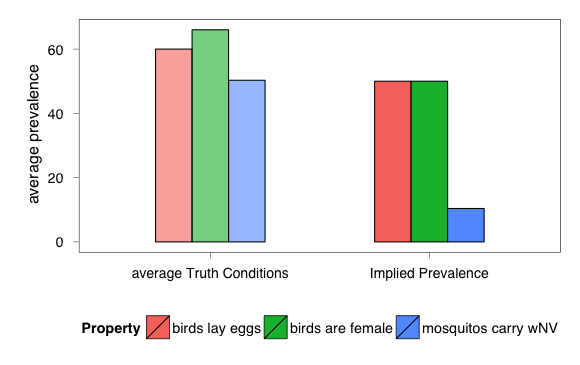
\includegraphics[width=0.8\columnwidth]{schematic_asym}
%  \end{center}
%  \caption{Schematic implied prevalence for generics like ``Birds lay eggs'', ``Birds are female'', and ``Mosquitos carry West Nile Virus''.}
%   \label{fig:schem_ip}
%\end{figure}



\section{Experiment 1: CBG -- primary findings replication}

The lifted-threshold RSA model predicts different truth conditions for generics when the prevalence prior differs. A paradigm was developed by \citeA{Cimpian2010} to get at a similar question. CBG also was concerned with determining whether or not the truth conditions for and implications from generic statements were comparable. To flesh out the motivation for the second question: consider sentences with the quantifier ``All'' (e.g. ``All lorches have purple feathers''). Presumably, this sentence is true only when 100\% of lorches have purple feathers. Similarly, upon hearing such an utterance, one is likely to infer that 100\% of lorches have purple feathers. CBG tested this symmetry with the quantifier ``most''--- ``the quantifier that comes closest to capturing generic meaning \cite{Carlson1977,Cimpian2010b}''. They found that participants judged ``most'' sentences true when between 50-100\% of the category had the property. Similarly, upon hearing an utterance with ``most'', participants on average inferred a prevalence of about 75\%. Thus, ``most'' also retains this symmetry as well. CBG found that generic statements, however, are judged true for a wide range of prevalence levels, but upon hearing a generic utterance, participants were likely to infer that \emph{all} or \emph{almost all} of the category had the property. Thus, the generic shows an \emph{asymmetry} between truth conditions and implications.


%That is, when the property in question was dangerous and distinct, participants required a lower overall prevalence (e.g. 10\% of lorches had purple feathers) to assert that the generic statement was true.

Experiment 1 attempted to replicate the main findings of CBG: that the type of property affects the proportion of ``true'' responses to a generic statement (Exp. 1a) and that there is an asymmetry between truth conditions and implications of the generic (Exp. 1b). 
%Exp. 1a and 1b were conducted on separate sessions, one week apart. None of the participants completed both experiments.

\subsection{Experiment 1a: \emph{truth conditions}}

In CBG's \emph{truth conditions} task, participants are given an evidence statement consisting of the percentage of a novel animal category that had a property (e.g.~``30\% of lorches have purple feathers''). Participants were asked to judge the associated generic statement (i.e.~``Lorches have purple feathers'') as true or false. 

Following CBG, we manipulated both the prevalence and the type of property within-subjects. Prevalence varied between 10, 30, 50, 70, and 90\%. Property type was manipulated by adding additional sentences to the prompt. CBG's original study used three property types: \emph{dangerous and distinct} (e.g.~``These feathers are as sharp as needles and can easily get lodged in you, causing massive bleeding. No other animals have these kinds of feathers.''), \emph{nondangerous and nondistinctive} (e.g.~``These feathers are wide and very smooth to the touch. Other animals have these kinds of feathers.''), and \emph{plain} (no additional statements). 

CBG found that proportion of ``true'' responses increased monotonically as prevalence increased. They also found an interaction with type: \emph{dangerous and distinctive} property had higher proportions of ``true'' responses to the generic, particularly so at lower prevalence levels. 

\subsubsection{Participants}

We recruited 40 participants over Amazon's crowd-sourcing platform Mechanical Turk (MTurk).  Participants were restricted to those with US IP addresses and with at least a 95\% MTurk work approval rating. All participants were native English speakers. The experiment took about 5 minutes and participants were compensated \$0.50.

\subsubsection{Procedure and materials}

Our procedure was very similar to CBG's \emph{truth conditions} task. Participants were told they were the resident zoologist of a team of scientists that recently discovered an island with many new animals; their task was to provide their expert opinion on questions about these animals\footnote{The experiment in full can be viewed at \url{http://stanford.edu/~mtessler/experiments/generics/cbg2010-replication/experiment/experiment-9.html}}. 

 %Our instructions were elaborated to improve interest and motivation
 
We used the same materials as CBG (available in their Appendix). The materials used were 30 novel animal categories (e.g. lorches, morseths, blins) each paired with a unique property. Properties were made by pairing a color with a body-part (e.g. purple feathers, orange tails). Each participant saw 30 unique animal-property pairs: 10 of each of the 3 types (\emph{dangerous and distinct}, \emph{nondangerous and nondistinct}, \emph{plain}). The 10 items of each property-type were randomly paired with 1 of 5 ``prevalence levels'': \{10, 30, 50, 70, 90\}\%; thus, each prevalence level appeared 2 times per type. 

On each trial, participants saw a prevalence statement and type statements (\emph{dangerous and distinct}, \emph{nondangerous and nondistinct}, \emph{Plain}; illustrated above). 
%A context here was either (1) dangerous \& distinct statements (e.g. ``These feathers are as sharp as needles and can easily get lodged in you, causing massive bleeding. No other animals have these kinds of feathers.''), (2) not distinct \& irrelevant statements (e.g. ``These feathers are wide and very smooth to the touch. Other animals have these kinds of feathers.'', or (3) nothing else. 
Participants were then asked ``Is the following sentence true or false?'', below which was presented the associated generic (e.g. ``Lorches have purple feathers'') and ``True'' and ``False'' radio buttons. 

\subsubsection{Results}


%\begin{figure}
%        \centering
%        \begin{subfigure}[t]{0.53\columnwidth}
%                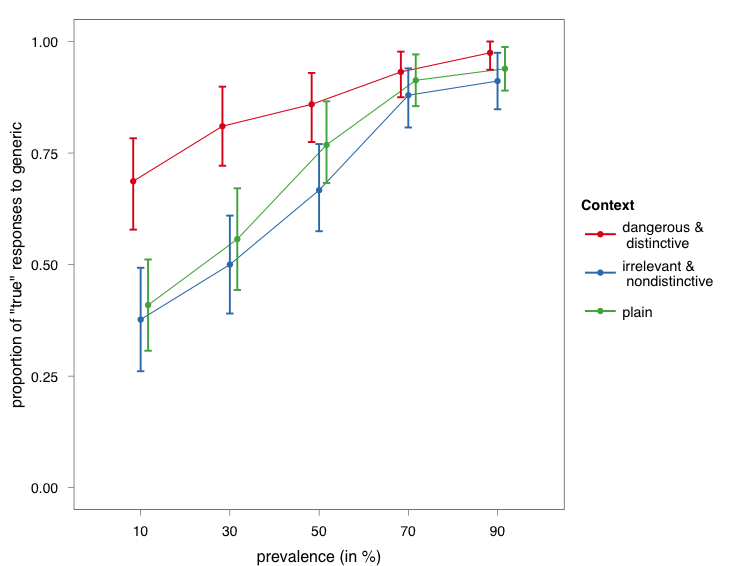
\includegraphics[width=\columnwidth]{data_truthconditions1}
%                \caption{Truth conditions of the generic vary across contexts. Error bars denote bootstrapped 95\% confidence intervals.}
%                \label{fig:datatc}
%        \end{subfigure}%
%        ~ %add desired spacing between images, e. g. ~, \quad, \qquad, \hfill etc.
%          %(or a blank line to force the subfigure onto a new line)
%        \begin{subfigure}[t]{0.42\columnwidth}
%                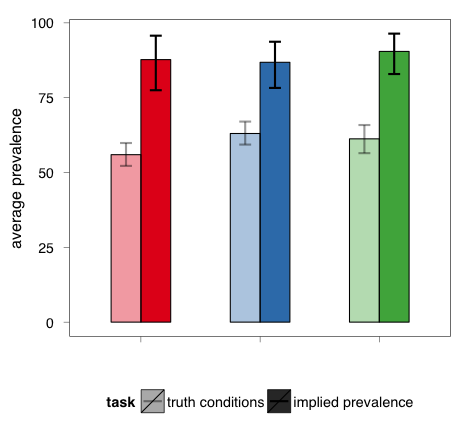
\includegraphics[width=\columnwidth]{data_asymmetry1}
%                \caption{Asymmetry between verification and interpretation, see text for details.}
%                \label{fig:datasym}
%        \end{subfigure}
%        ~ %add desired spacing between images, e. g. ~, \quad, \qquad, \hfill etc.
%          %(or a blank line to force the subfigure onto a new line)
%        \caption{Replication of CBG}\label{fig:exp1}
%\end{figure}

\begin{figure}
\centering
    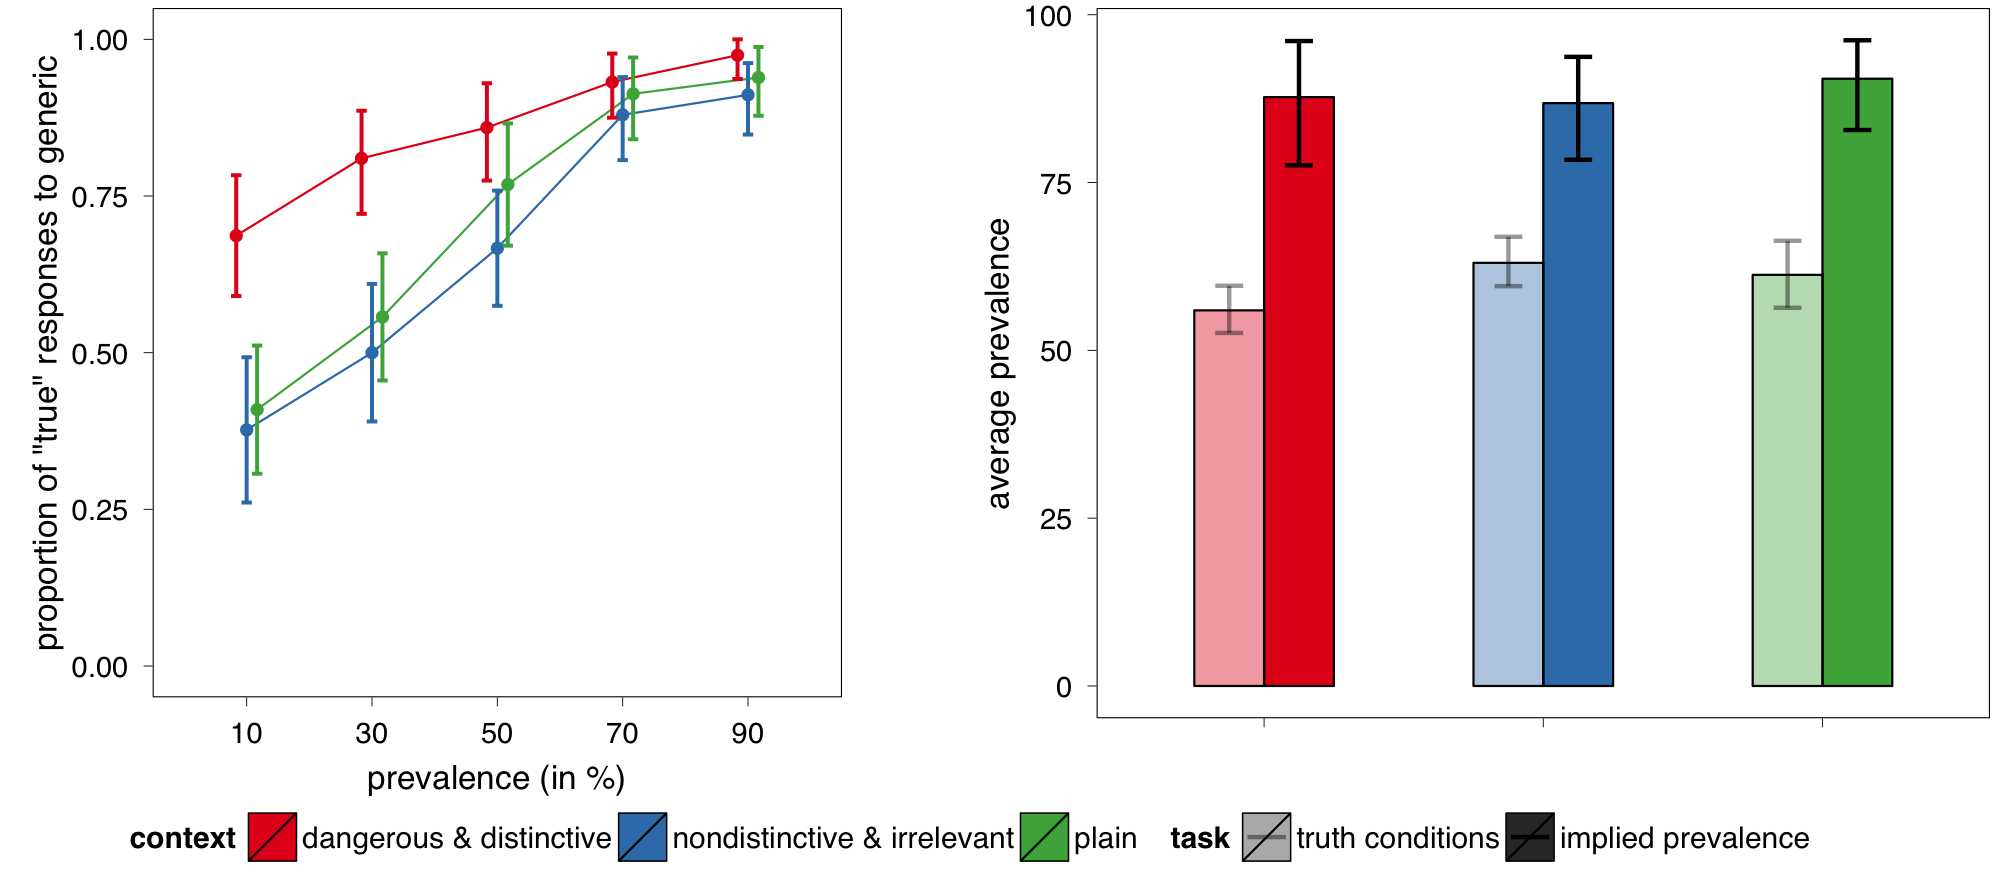
\includegraphics[width=\columnwidth]{Xexp1data}
    \caption{Replication of CBG. Left: \emph{truth conditions} vary by context (Exp. 1a). Right: \emph{implied prevalence} of the generic is greater than \emph{truth conditions} (Exp. 1b). Error bars denote bootstrapped 95\% confidence intervals.}
  \label{fig:exp1}
\end{figure}

Results are shown in Figure~\ref{fig:exp1} (Left). We entered participants' truth judgments into a mixed effects logistic regression with random by-item and by-participant effects of intercept and fixed effects of prevalence and type as well as their interaction\footnote{This was the maximal mixed-effect structure supported by the data.}.  
%
Our results replicated the finding of CBG that the generic statements were endorsed more with dangerous and distinctive properties than with plain properties (Figure \ref{fig:exp1}, left; $\beta=1.99; SE = .36; z = 5.52; p < .001$). 
%
There was also an interaction between prevalence level and type such that the generic was endorsed more with \emph{dangerous and distinctive} properties than with plain properties at lower prevalence levels ($\beta=.03; SE = .01; z=2.35; p = 0.019$). There was a trending effect for the \emph{nondangerous and nondistinct} properties to be endorsed \emph{less} than the plain properties ($\beta=-.57; SE = .30; z=-1.91; p = .056$).

\subsection{Experiment 1b: \emph{implied prevalence}}

In their \emph{implied prevalence} task, participants were supplied with the generic and asked to judge prevalence: ``What percentage of lorches do you think have purple feathers?''. Type was again manipulated within-subject. CBG found that the generic was interpreted strongly---nearly all lorches have purple feathers---for all three types of properties.

\subsubsection{Participants}

We recruited 30 participants over MTurk\footnote{This study was ran 1 week after Exp. 1a. None of the participants in Exp. 1a participated in Exp. 1b.}.  Participants were restricted to those with US IP addresses and with at least a 95\% MTurk work approval rating. All participants were native English speakers. The experiment took about 5 minutes and participants were compensated \$0.50.

\subsubsection{Procedure and materials}

Our procedure was very similar to CBG's \emph{implied prevalence} task. Our instructions were the same as in Exp. 1a\footnote{The experiment in full can be viewed at \url{http://stanford.edu/~mtessler/experiments/generics/cbg2010-replication/experiment/experiment-12.html}}. 

The materials and property-type conditions were the same as in Exp. 1a. Each participant saw 10 trials of each of the 3 property-types (30 trials in total). On each trial, participants saw a generic statement and property-type statements. 
%A context here was either (1) dangerous \& distinct statements (e.g. ``These feathers are as sharp as needles and can easily get lodged in you, causing massive bleeding. No other animals have these kinds of feathers.''), (2) not distinct \& irrelevant statements (e.g. ``These feathers are wide and very smooth to the touch. Other animals have these kinds of feathers.'', or (3) nothing else. 
Participants were then asked ``What percentage of [the kind] do you think have [the property]?'' (e.g. ``What percentage of lorches do you think have purple feathers?'') The dependent measure was a free response required to be an integer, $0-100$. 

\subsubsection{Data analysis and results}
\label{subsec:cbganalysis}

%\begin{figure}
%\centering
%    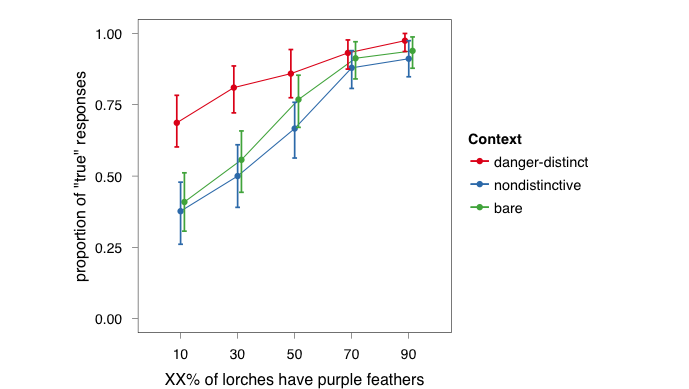
\includegraphics[width=\columnwidth]{fig1_replication}
%    \caption{Replication of CBG \emph{asymmetry}, generics condition}
%  \label{fig:replication}
%\end{figure}
%
To compare the truth conditions data with the implied prevalence data, we followed the data analysis strategy of CBG. Using the data from Exp. 1a, we computed, for each subject, an \emph{average prevalence level} that led to ``True'' responses. For example, if a participant said ``True'' whenever the prevalence was 70\% or 90\% and ``False'' to everything else, that participant received an \emph{average prevalence score} of 80\%; if a participant said ``False'' to everything, their \emph{average prevalence score} was 100\%, since they presumably were interpreting the generic statement as a universal (i.e. an ``all'' statement). This score was compared against the implied prevalence dependent measure of Exp. 1b. 

The prevalence scores from each task were entered into a linear mixed model with a by-participant random effect of intercept; the fixed effects were property-type, task, and their interaction. Our results replicated the asymmetry finding of CBG that the generic statement was interpreted as having a higher prevalence than its truth conditions entail (i.e. main effect of task; $\beta=28.8; SE = 4.3; t=6.6; p < 0.001$; see Fig.~\ref{fig:exp1}, right). In the original study, this asymmetry was not observed for sentences using the quantifier ``most''; however, we did not replicate this effect here.

%    \section{Threshold semantics}
%    The above results, replicated from CBG, indirectly constrain the effective truth conditions that participants are using for generic statements within these experimental conditions. In this section, we briefly review threshold semantics and the trouble posed by this data.
%    
%    Let us assume that the conditions for truth of the generic can be usefully represented by a threshold on prevalence: the generic is true when the prevalence of some property within a kind exceeds a given threshold (see \citeA{Cohen1999} for a similar assumption). If we use $x\in [0,1]$ to denote the prevalence $P(\text{property}|\text{category})$, then the simple threshold meaning is:
%    
%    \begin{align}
%     g(x, \theta) = \begin{cases}
%       1 & \text{if } x > \theta \\
%       0       & \text{if } x \leq \theta
%      \end{cases}
%    %  \tag{\theequation}
%       \label{eq:ftsem}
%    \end{align}
%    
%    The function $g$ captures a very simple cognitive model in which people evaluate the generic by comparing observed prevalence to the known threshold.
%    It is apparent that if the threshold $\theta$ were truly fixed, this model could account for neither property-type nor asymmetry effects.
%    
%    The simplest model that could account for context effects would one in which the threshold was a function of context. 
%    
%    
%    \subsection{A context-dependent fixed-semantics}
%    
%    We reexamine our fixed-semantics model, now allowing for the possibility that $\theta$ could vary by property-type: $g(x,\theta_{type})$.
%    
%    To begin our data analysis, we make no \emph{a priori} assumptions about the (fixed, but unknown to us) values of $\theta_{type}$, placing on it a uniform prior distribution: $\theta_{type} \thicksim U(0,1)$. 
%    We account for inattention and other irrelevant factors by including a probability $\phi_{task}\thicksim U(0,1)$ for each task that a given response is the result of uniform random guessing\footnote{Ideally, we would have $\phi$ be a function of participant (some participants guess more than others) and experimental condition (some conditions are more difficult or less constrained and invite more guessing). This is computationally too demanding when coupled with the more complex cognitive model explored later.}  \cite{LW2014}.
%    The inferred ``guessing'' parameter $\phi$ is the amount of data that would have to be attributed to random guessing in order for the fixed-threshold model of the generic to apply to the experimental data. In this sense, $\phi$'s provide a coarse notion of model fit. 
%    
%    %We attach uniform priors to each of the $\theta_{c}$'s to examine the data from the two experiments. . 
%    
%    We are now in a position to examine how a truth-functional threshold of the generic would need to behave across these three contexts. 
%    
%    %\subsubsection{Inferred parameters}
%    
%    The results can be seen in Figure \ref{fig:justFixed}. 
%    The posterior distributions for $\phi_{t}$'s show that the amount of data that must be attributed to guessing to be consistent with this model of generics is still quite high: around 45\% for the \emph{truth conditions} task. 
%    Turning to $\theta_{c}$, there is evidence for the variability of the generic threshold in the \emph{truth conditions} task. In the \emph{plain} context, the analysis suggests the threshold is somewhere between 0\% and 30\%, but it's unclear where exactly in that range the threshold should be. Critically, in the \emph{dangerous and distinctive} context, the analysis infers a lower threshold, less than 10\%. This matches with the earlier Null Hypothesis analysis. Finally, and most intriguingly, the analysis infers a third distinct threshold profile for the \emph{nondistinctive and irrelevant} context.  The inferred threshold is greater than 10\%, but could be as high as 50\%. This is an overall higher inferred threshold for the nondistinctive category; however, these results are inconclusive as to whether or not this threshold is actually different from the \emph{plain} context.
%    
%    
%    
%    \begin{figure}
%    \centering
%        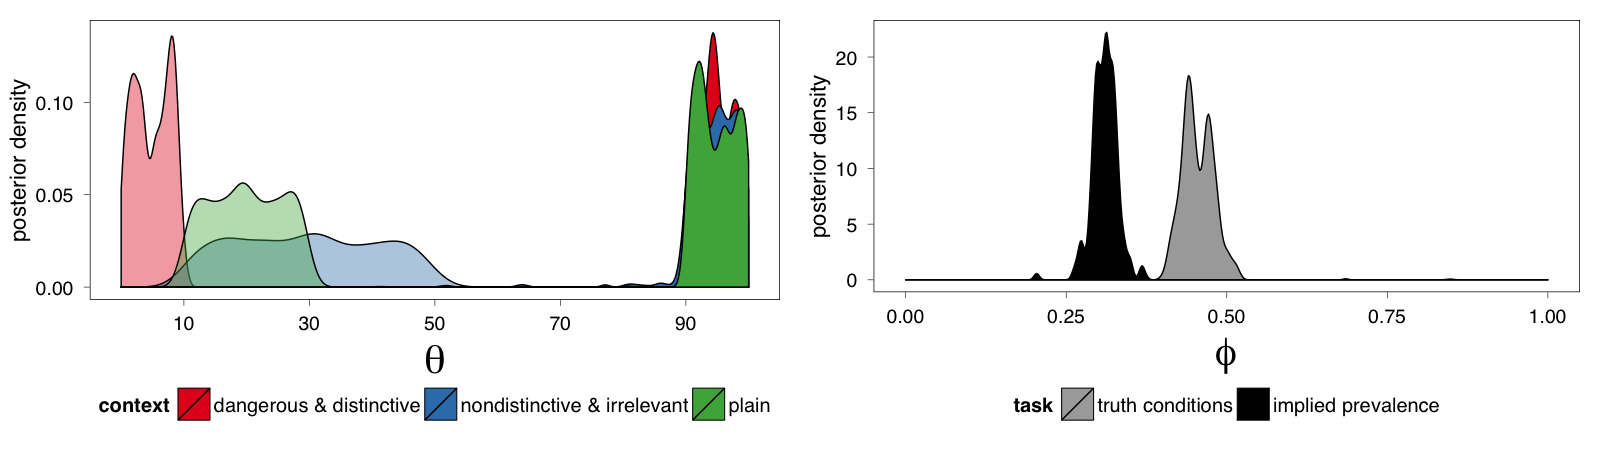
\includegraphics[width=\columnwidth]{fixed_phis_thetas}
%        \caption{Analysis of the context-dependent fixed-semantics of a generic. Left: Inferred threshold for each experiment and context. Right: ``guessing'' parameter for each experiment.}
%      \label{fig:justFixed}
%    \end{figure}
%    
%    
%    
%    
%    %\subsubsection{Posterior predictives}
%    
%    The fixed-semantics model can also be evaluated by examining the posterior predictive distribution of responses. 
%    The posterior predictive distribution marginalizes over the inferred parameter values to produce predictions about what the data should look like given the cognitive model and the observed data. This is akin to fitting the parameters and is an important step in model validation as it shows what data is actually predicted by the model.
%    %\footnote{As a thought experiment, consider 2 coins assumed to come from a single coin-making machine (all the coins from this machine have the same weight). You flip each coin 100 times. The first one returns 100 heads, and the second one returns 100 tails. The posterior mean of the inferred coin weight will be 0.5. Comparing the posterior predictive distribution (based on this inferred coin-weight) to the observed data, however, will highlight the fact that your theory about the ``single coin-making machine'' is seriously flawed.}.
%    Following directly from the inferred $\theta_{c}$'s, the model matches the ordering of the truth-conditions by context reasonably well. However, the model predicts an abrupt transition in endorsement rates for prevalences on either side of the threshold; the model is too dichotomous to match the human data. The correlation between the posterior predictive and the data is a moderate $r = 0.81$. 
%    
%    The fixed-threshold semantics model is not flexible enough to explain the observed data, but it has an even more serious flaw: the variation of threshold by condition is postulated \emph{a priori} in the data analysis, rather than accounted for by the cognitive model. That is, participants in our experiment must have some way of arriving at different thresholds for different tasks and conditions, which this model has no means to explain. For a more explanatory model we turn to the pragmatics of language understanding.

%
%
%
%To set the stage for future Bayesian analyses, let us nonetheless explore the quantitative relation of a context-invariant threshold semantics to the data.
%
%\subsection{A context-invariant fixed-semantics}
%%We first examine what this threshold would look like if it were invariant to context and task. 
%To begin our data analysis, we make no \emph{a priori} assumptions about the (fixed, but unknown to us) value of $\theta$, placing on it a uniform prior distribution: $\theta \thicksim U(0,1)$. 
%We account for inattention and other irrelevant factors by including a probability $\phi_{t}\thicksim U(0,1)$ for each task that a given response is the result of uniform random guessing\footnote{Ideally, we would have $\phi$ be a function of participant (some participants guess more than others) and experimental condition (some conditions are more difficult or less constrained and invite more guessing). This is computationally too demanding when coupled with the more complex cognitive model explored later.}  \cite{LW2014}.
%The inferred ``guessing'' parameter $\phi$ is the amount of data that would have to be attributed to random guessing in order for the fixed-threshold model of the generic to apply to the experimental data. In this sense, $\phi$ gives a coarse notion of model fit. 
%%We analyze the data from Exp. 1a and 1b jointly as well as independently.
%
%
%%Following standard practice in Bayesian data analysis \cite{LW2014}, we include the data-analytic parameter $\phi$ to account for data points that deviate strongly from our theory; it is a guessing parameter. We assume there is some proportion of responses where the participant is responding randomly, and we estimate this quantity by way of $\phi$. We model two such $\phi$ parameters, one for each task.
%%
%%\begin{align*}
%%\theta \thicksim U(0,1) \\
%%\phi_{t} \thicksim U(0,1) %\mid  t \in \{exp1a, exp1b\}
%%\end{align*}
%
%
%%We formalize the notion of ``effective truth conditions'' by saying the generic is a function from states of the world to truth-values. We operationalize \emph{states of the world} here as the prevalence of some property within a kind. This mapping is then determined by some threshold such that the generic is true when the prevalence is above threshold. 
%
%%Using the Church probabilistic programming language to represent this model \cite{probmods}, this would be written:
%%
%%\begin{lstlisting}
%%(define generic 
%%	(lambda (prevalence) (> prevalence generic-threshold)))
%%\end{lstlisting}
%
%%To handle the inference problem the participant is faced with, we express the subject's uncertainty about whether the generic is true or false.
%%
%%\red{NDG: the rest of this section is too long and doesn't make sense to me...}
%% \begin{lstlisting}
%%(define truth-conditions (lambda (prevalence)
%%	(query  
%%	
%%		(define generic ...) ;defined as above
%%		(define generic-is-true? (flip 0.5))
%%		
%%		generic-is-true?
%%			
%%		(generic prevalence))))
%%\end{lstlisting}
%
%
%
%%\subsubsection{Inferred parameters}
%
%
%
%A joint analysis of the data from Exp. 1a and 1b, produces the expected extreme results. The inferred $\phi_{1a}$ is near 1, $\phi_{1b}$ has a more reasonable posterior mean of 0.3, and the inferred $\theta$ is near 100\%. That is, the best interpretation of the data discounts the \emph{truth conditions} data entirely and uses only the \emph{implied prevalence} data to set the threshold, which results in interpreting the generic as a universal quantifier.
%A separate by-experiment analysis produces thresholds that are completely different for the two tasks. 
%For the implied prevalence task, the threshold is again close to 100\%. 
%For the truth conditions task, the threshold is probably greater than 10\% and less than 30\%\footnote{This uncertainty results from the sparseness of our measure: participants were queried only at prevalence levels 10, 30, 50, 70, and 90\%.}.
%
%%The amount of guessing for the \emph{truth conditions} task ($\phi_{1a}$) is no longer near 1, but is still quite high, around 0.5, which means that participants would have to be guessing 50\% of the time. Though this analysis shows an asymmetry between the two tasks, it doesn't have the ability to capture the context-dependence present in the data. 
%%we already know there is an effect of context on the generic meaning. There is no way for this model to account for such data.
%
%%\begin{figure}
%%\centering
%%    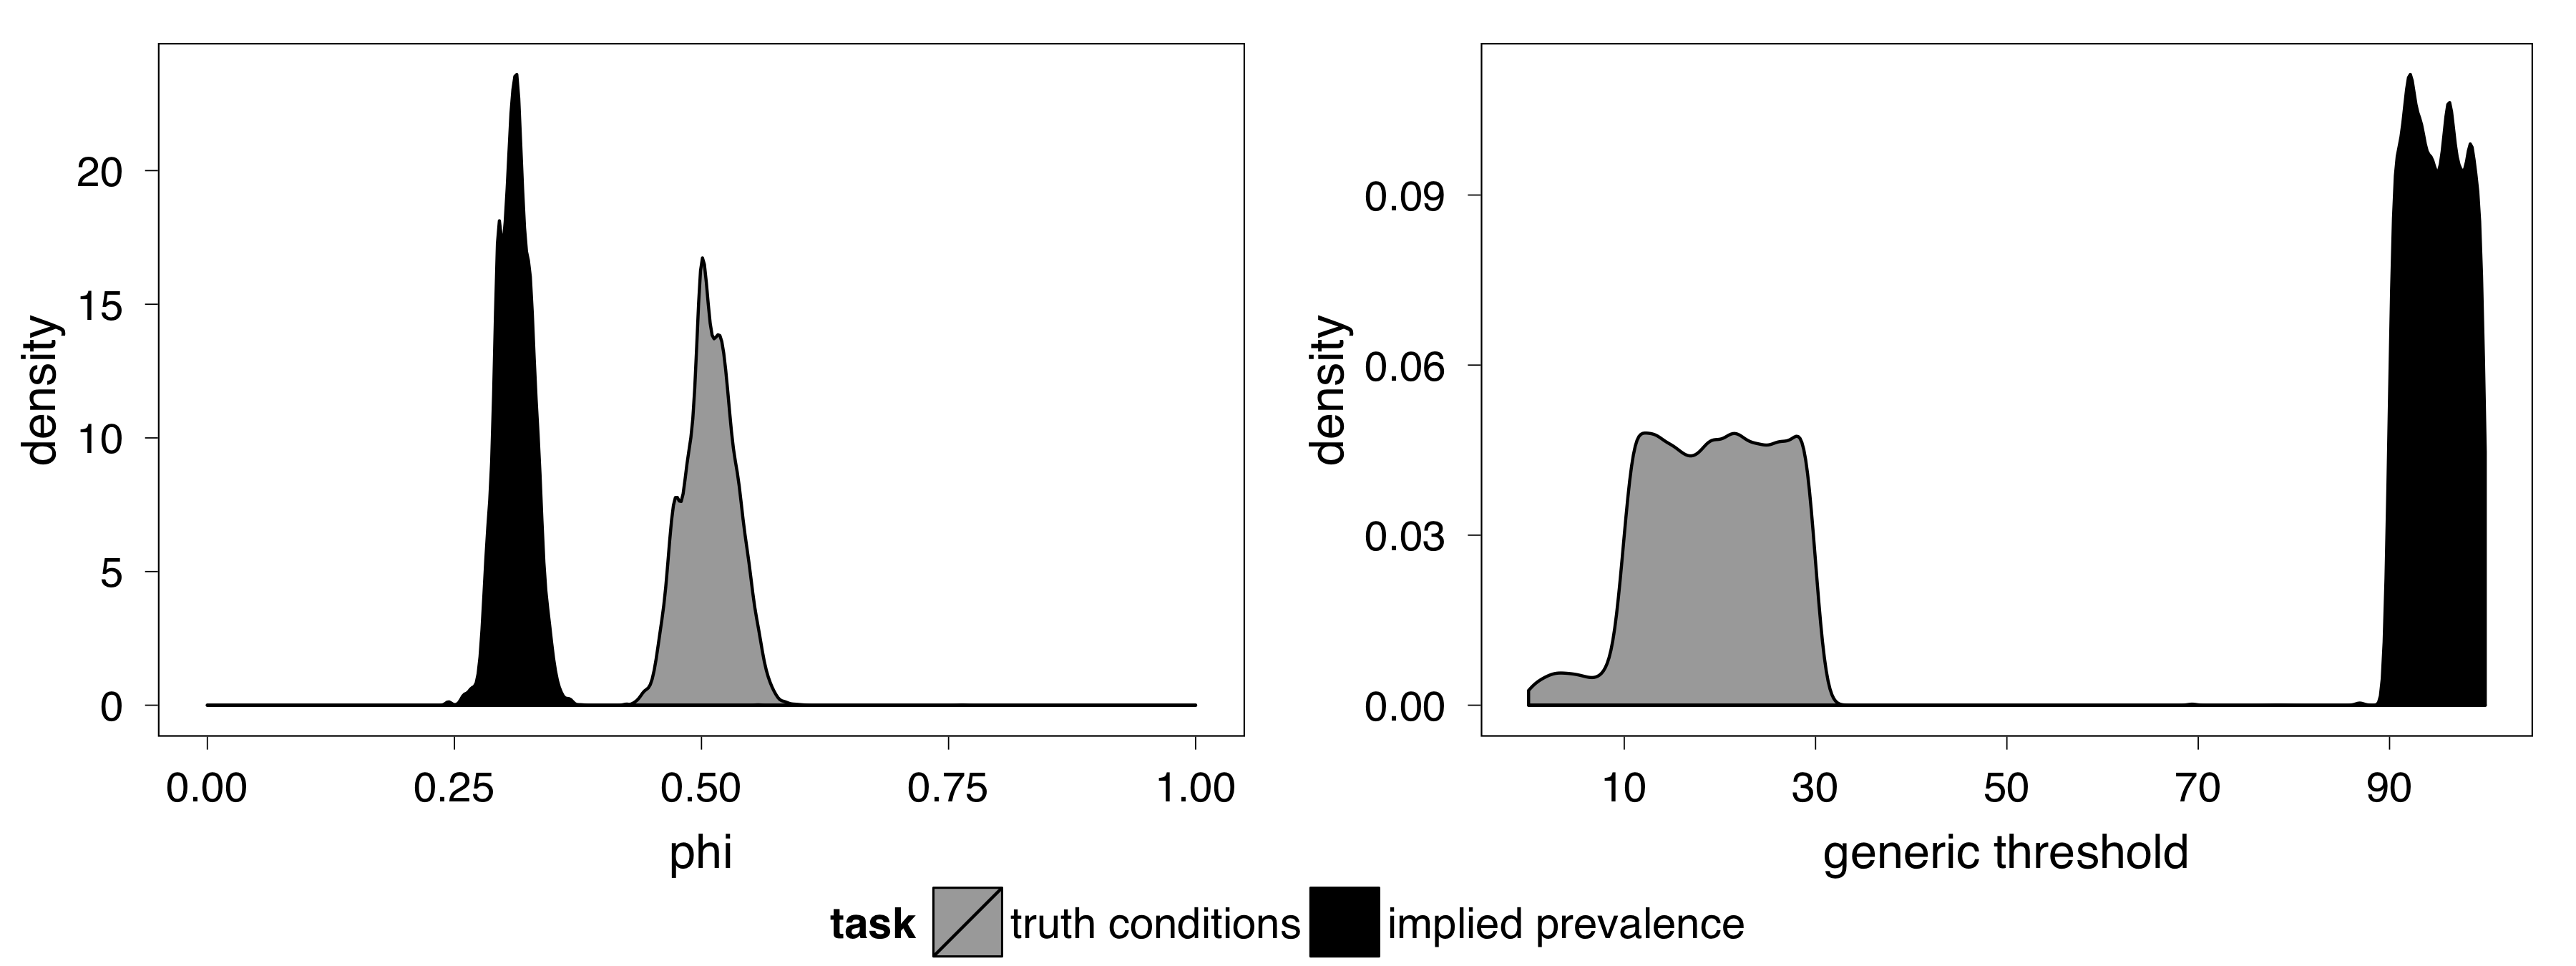
\includegraphics[width=\columnwidth]{trulyFixed_phis_thetas}
%%    \caption{Fixed and context-invariant semantics of a generic. Inferred ``guessing'' parameter (left) and threshold (right) for each experiment.}
%%  \label{fig:trulyfixed}
%%\end{figure}
%
%


\section{Model analysis}

\begin{figure}
\centering
    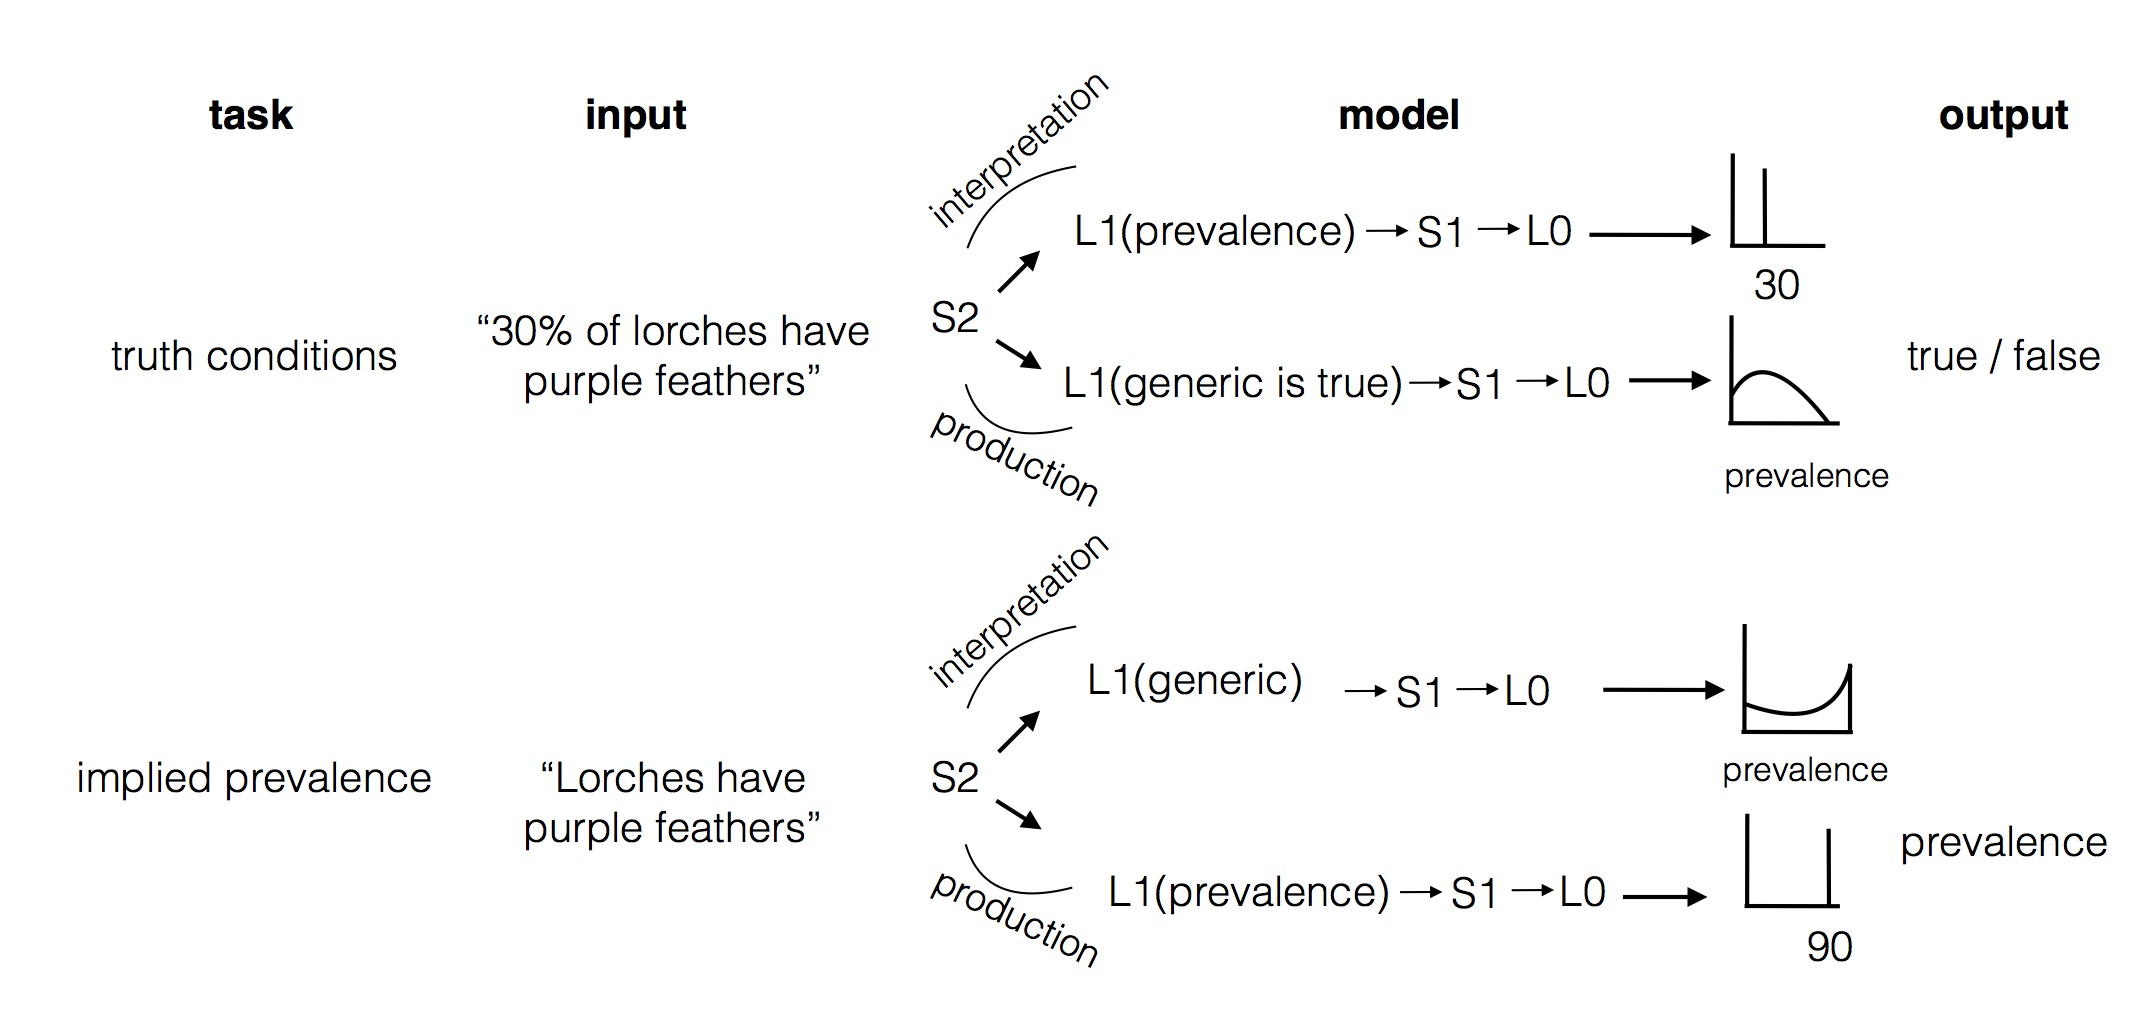
\includegraphics[width=\columnwidth]{model_schematic}
    \caption{Schematic of the input--output structure of the model.}
  \label{fig:model}
\end{figure}

A schematic of the model and our linking assumptions is shown in Figure \ref{fig:model}. We model the \emph{truth conditions} task as a speaker who can either say ``[[the generic]] is true'' or ``[[the generic]] is false'', as we did in Section \ref{sec:simulations}. This speaker could also be thought of as having a second $L_{1}$ branching off from her, charged with interpreting the prevalence statement given in the task (e.g. ``30\% of lorches have purple feathers''). This submodel would reduce to a delta function, as the utterance (``30\% ...'') is completely unambiguous and maps directly onto a prevalence level (i.e. ``30\%'').

We model the \emph{implied prevalence} task also as an $S_{2}$. Just like the participant in the task, this model takes the generic as input. The generic then gets passed immediately down to the $L_{1}$ listener, who does lifted-threshold inference to determine the right interpretation. The \emph{implied prevalence $S_{2}$} then says which prevalence is most likely to be the case. This ``prevalence utterance'' gets passed down to an $L_{1}$. Like the prevalence $L_{1}$ in the \emph{truth conditions} model, this submodel reduces to a delta function (i.e. responding ``90\% of lorches have purple feathers'' means that 90\% of lorches have purple feathers)\footnote{N.B.: This model as a whole is equivalent to just the pragmatic listener ($L_{1}$) model that is trying to infer the prevalence.}. We articulate both models as $S_{2}$s to highlight the similarities between them.


\subsection{Bayesian model evaluation}
\label{sec:model1}

As a first test of our lifted-threshold model of generics, we posit a family of possible priors over the prevalence $x \thicksim \beta(\gamma,\delta)$\footnote{For ease of interpretation, we are parametrizing the $\beta$ distribution by its mean and concentration. To recover the canonical shape parametrization, use $\gamma \delta$ and $(1-\gamma)\delta$.}. We hypothesize that the details of these priors (i.e.~$\gamma$'s and $\delta$'s) may differ according to the type of property in reference by the generic. For instance, when you know that a particular property is rare, a different prior distribution of that property over kinds (i.e. a different prevalence prior) is called to mind, than if the property is common. This would result in different meanings for the generic. Below we infer appropriate prior parameters for each property-type from the behavioral data.

%To evaluate our lifted-threshold model of generics we perform a Bayesian data analysis similar to that used above.
%to evaluate this more sophisticated cognitive model. We are interested in how the hyperprior parameters $\gamma$ and $\delta$ might vary across contexts.
We infer the parameters of the prevalence prior, $\beta(\gamma,\delta)$ using uninformative hyperpriors:
%
%$\gamma_{type} \thicksim U(0,1)$,  $\delta_{c} \thicksim U(0,5)$, $\phi_{t} \thicksim U(0,1)$,
\begin{align*}
\gamma_{type} \thicksim U(0,1) \\
\delta_{type} \thicksim U(0,5) \\
\phi_{task} \thicksim U(0,1) \\
\lambda_{task} \thicksim U(0,5)
\end{align*}

where $type \in \{$dangerous and distinct, nondangerous and nondistinct, plain$\}$ and $task \in \{$truth conditions, implied prevalence$\}$.

We account for inattention and other irrelevant factors by including a probability $\phi_{task}\thicksim U(0,1)$ for each task that a given response is the result of uniform random guessing\footnote{Ideally, we would have $\phi$ be a function of participant (some participants guess more than others) and experimental condition (some conditions are more difficult or less constrained and invite more guessing). This is computationally too demanding when coupled with the complex cognitive model explored here.}  \cite{LW2014}.
The inferred ``guessing'' parameter $\phi$ is the amount of data that would have to be attributed to random guessing in order for our cognitive model of the generic to apply to the experimental data. In this sense, $\phi$ gives a coarse notion of model fit. 

%Following standard practice in Bayesian data analysis \cite{LW2014}, we include the data-analytic parameter $\phi$ to account for data points that deviate strongly from our theory; it is a guessing parameter. We assume there is some proportion of responses where the participant is responding randomly, and we estimate this quantity by way of $\phi$. We model two such $\phi$ parameters, one for each task.



%We propose that, in this paradigm, nobody knows $\theta$.  $\theta$ is influenced by the prior distribution over prevalence, which in turn is influenced by the contextual information provided (\emph{DD}, \emph{NI}, or \emph{P}). This contextual information could imply different $P(x)$, prior probability distributions over the prevalence of a property. 
%
%Naively, this distribution would be $U(0,1)$, or equivalently, $\beta(1,1)$. However, we propose that people have different prior distributions in mind, depending on features of the properties under discussion (e.g. distinctiveness).
%
%Although we might have some intuitions what these prior distributions might look like, we put uncertainty over the parameters of this Beta distribution $\beta(\gamma,\delta)$, outside of the RSA model but inside of the data analysis model. 
%
%\begin{align*}
%x_{c} \thicksim \beta(\gamma_{c},\delta_{c}) \\
%\gamma_{c} \thicksim U(0,1) \\
%\delta_{c} \thicksim U(0,5) \\
%\phi_{t} \thicksim U(0,1) 
%\end{align*}
%
%Here, $c \in \{DD,NI,P\}$ and $t \in \{$truth conditions, implied prevalence$\}$.
%
%Thus, we do Bayesian data analysis on a Bayesian Rational Speech-Act model of language understanding, to see how context might influence the prior distribution given the data we've observed. We keep the data-analytic guessing parameters $\phi_{t}$ as a gross estimate of the proportion of responses our model of cognition doesn't capture. 

%    \begin{wrapfigure}{l}{0.5\columnwidth}
%    \vspace{-16pt}
%     \begin{center}
%    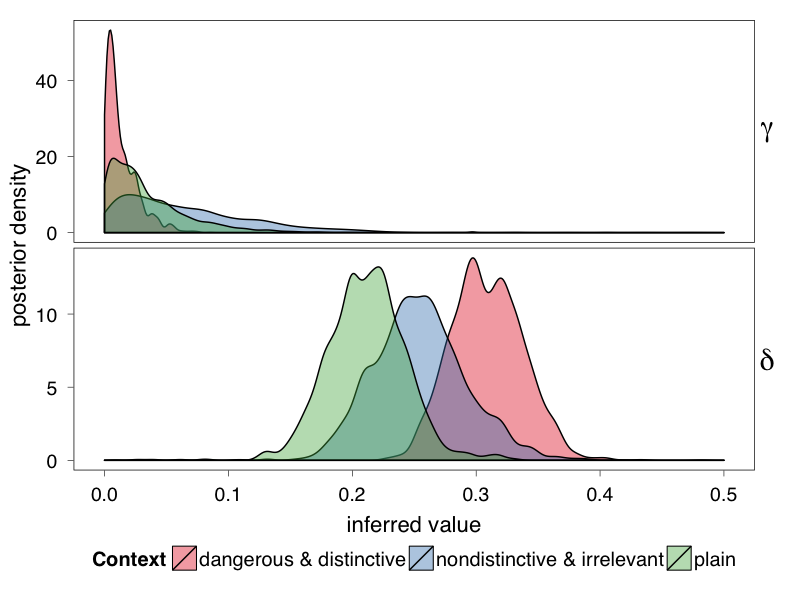
\includegraphics[width=0.48\columnwidth]{inferred_hyperpriors}
%     \end{center}
%     \caption{Posterior distributions of the hyperprior parameters used in lvRSA.}
%    label{fig:posthyper}
%    \end{wrapfigure}
%    

%\begin{wrapfigure}{l}{0.5\columnwidth}
%  \begin{center}
%    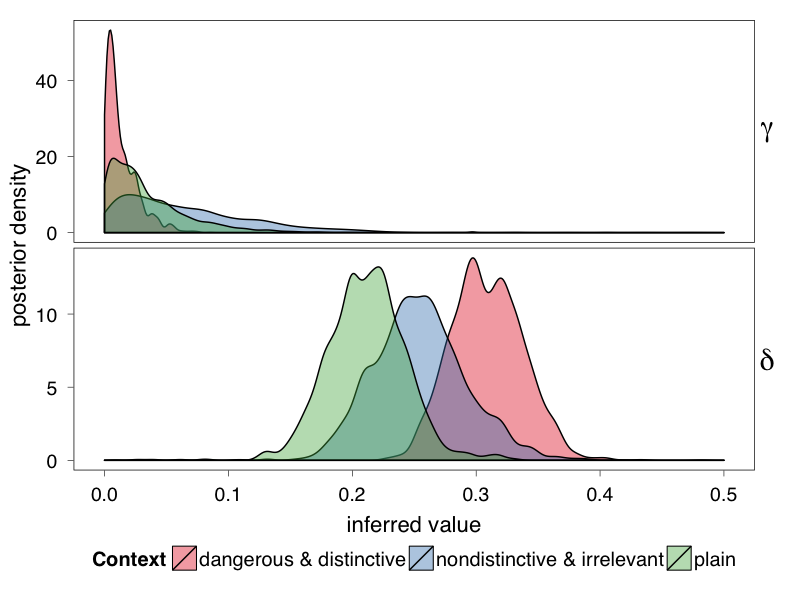
\includegraphics[width=0.48\columnwidth]{inferred_hyperpriors}
%  \end{center}
%  \caption{Posterior distributions of the hyperprior parameters used in lvRSA.}
%   \label{fig:posthyper}
%\end{wrapfigure}


\begin{figure}
\centering
    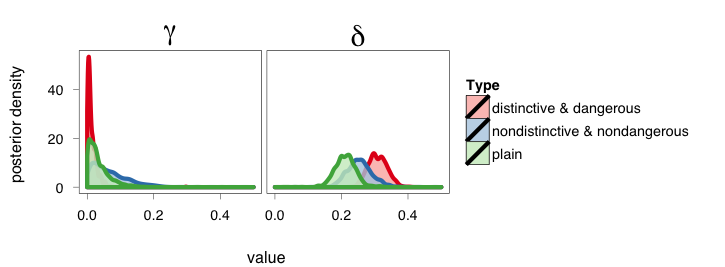
\includegraphics[width=\columnwidth]{lvRSA_hyperparams_sidebyside}
  \caption{Posterior distributions of the hyperprior parameters used in the lifted-threshold generics model. Gamma is .... Delta is ...}
   \label{fig:posthyper}
\end{figure}

\subsubsection{Inferred parameters}
The mean inferred values of  $\phi_{1a}$ and $\phi_{1b}$ are about 0.08 and 0.05, respectively, a reasonable rate of ``guessing'' for participants on Amazon's Mechanical Turk. This also  indicates that our model of cognition is doing a good job at accounting for the signal in participants' responses (i.e., it's better than a model of random guessing). The Maximum A Posteriori (MAP) inferred values for the rationality parameters $\lambda_{truth}$ and $\lambda_{implied}$ were approximately 1 and 2, respectively. 

%We use Bayesian data analysis to infer the values of the hyperprior parameters $\gamma$ and $\delta$ for the Bayesian lvRSA model. 

Figure \ref{fig:posthyper} shows the posterior distributions of the hyperprior parameters, $\gamma$ and $\delta$, for the lifted-threshold RSA model. The posterior means for the hyperparameters $\gamma_{type}$ are well-ordered: dangerous \& distinct $<$ plain $<$ nondangerous and nondistinct. $\gamma_{type}$ reflects the mean of the prevalence prior. Thus, this can be directly interpreted as the mean prior prevalence for the three property types: \emph{dangerous and distinctive} properties are more rare than the other two types of properties. 

Additionally, the $\delta$'s are much lower than 1 in each case, indicating bi-modal priors peaked at 0 and 1. This is consistent with all of the properties being construed as \emph{biological} properties. Biological properties have the feature of being almost universally present or almost univeraslly absent within a kind (e.g. ~100\% of birds have wings; ~0\% of humans have wings). The posterior means for the $\delta$'s are also ordered, suggesting that participants may treat variance of prevalence as higher for the \emph{dangerous and distinctive} properties (or simply be more confused).

An intuitive way to visualize these inferred hyperparameters is to marginalize over the posterior parameter values to reconstruct a ``canonical'' prior distribution over prevalence for each property type. Figure \ref{fig:inferredpriors} shows these prior distributions inferred from Exp. 1a \& 1b data via the lifted-threshold RSA model. 
Qualitatively, they are each bi-modal and the \emph{dangerous and distinctive} prior has a lower mean.


%\begin{wrapfigure}{r}{0.5\textwidth}
%\centering
%   \begin{center}
%    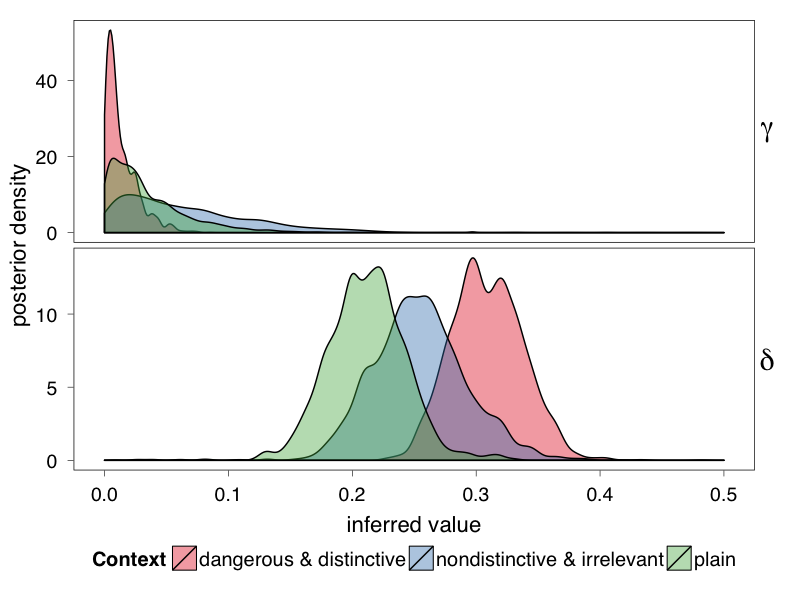
\includegraphics[width=0.48\columnwidth]{inferred_hyperpriors}
%    \end{center}
%    \caption{Posterior distributions of the hyperprior parameters used in lvRSA.}
%  \label{fig:posthyper}
%\end{wrapfigure}

%begin{table}[h]
%\centering
%\begin{tabular}{c | c | c}
%context / parameter & $\gamma$ & $\delta$ \\
%\hline
%DD                  & 0.016  & 0.321  \\
%NI                  & 0.054  & 0.245  \\
%P                   & 0.031  & 0.204 
%\end{tabular}
%\caption{Posterior means for hyperprior parameters.}
%\label{table:postmeans}
%\end{table}
%



\subsubsection{Posterior predictives}

We further evaluate the model by examining the posterior predictive distribution of responses. The posterior predictive distribution marginalizes over the inferred parameter values to produce predictions about what the data should look like given the cognitive model and the observed data. This is akin to fitting the parameters and is an important step in model validation as it shows what data is actually predicted by the model.

The posterior predictions by the lifted-threshold RSA model for the \emph{truth conditions} task are shown in Figure \ref{fig:lvRSAposteriorpred}. 
We can see that the model predicts monotonically increasing endorsement rates for the generic as a function of prevalence. The model has some persistent uncertainty about the true value of the threshold and this uncertainty is evident in the human behavior curves of Exp. 1a.
The model also matches the differences in endorsement rates between property-type conditions: dangerous and distinctive properties are endorsed more than the other two property types, and this difference dissipates at high prevalence levels.
We reconstruct the curves of Figure \ref{fig:exp1} reasonably well; the model--data correlation is $r = 0.90$.

%lvRSA models the \emph{truth conditions} task as a speaker---$S_{2}$ using Eq.~\eqref{eq:S2}---faced with the task of saying whether or not the generic applies to a given prevalence of a property. This utterance is intended for a pragmatic listener---$L_{1}$ using Eq.~\eqref{eq:L1}---who will try to reconstruct the prevalence that $S_{2}$ has observed. Here, we have modeled the \emph{implied prevalence} task as this listener, $L_{1}$, given the utterance, tasked with reconstructing the prevalence. 

We use a similar data analysis strategy as we did for Exp. 1b to compare ``average prevalence'' between truth conditions and implications. For the \emph{truth conditions} task, we used the model's posterior probability of saying ``true'' at each prevalence level to simulate trials of the experiment as Bernoulli trials. We simulated 30 trials for each of 1000 imaginary subjects in this way. We then followed CBG's data analysis strategy (as recapitulated in Exp.~1b). The model gives a posterior distribution over prevalences, whose expectation we used to model the \emph{implied prevalence} task. We find the model predicts the asymmetry between interpretation and verification of the generic for all three property types (see Figure \ref{fig:lvRSAposteriorpred}, right).

%\subsubsection{Discussion}

\begin{figure}
\centering
    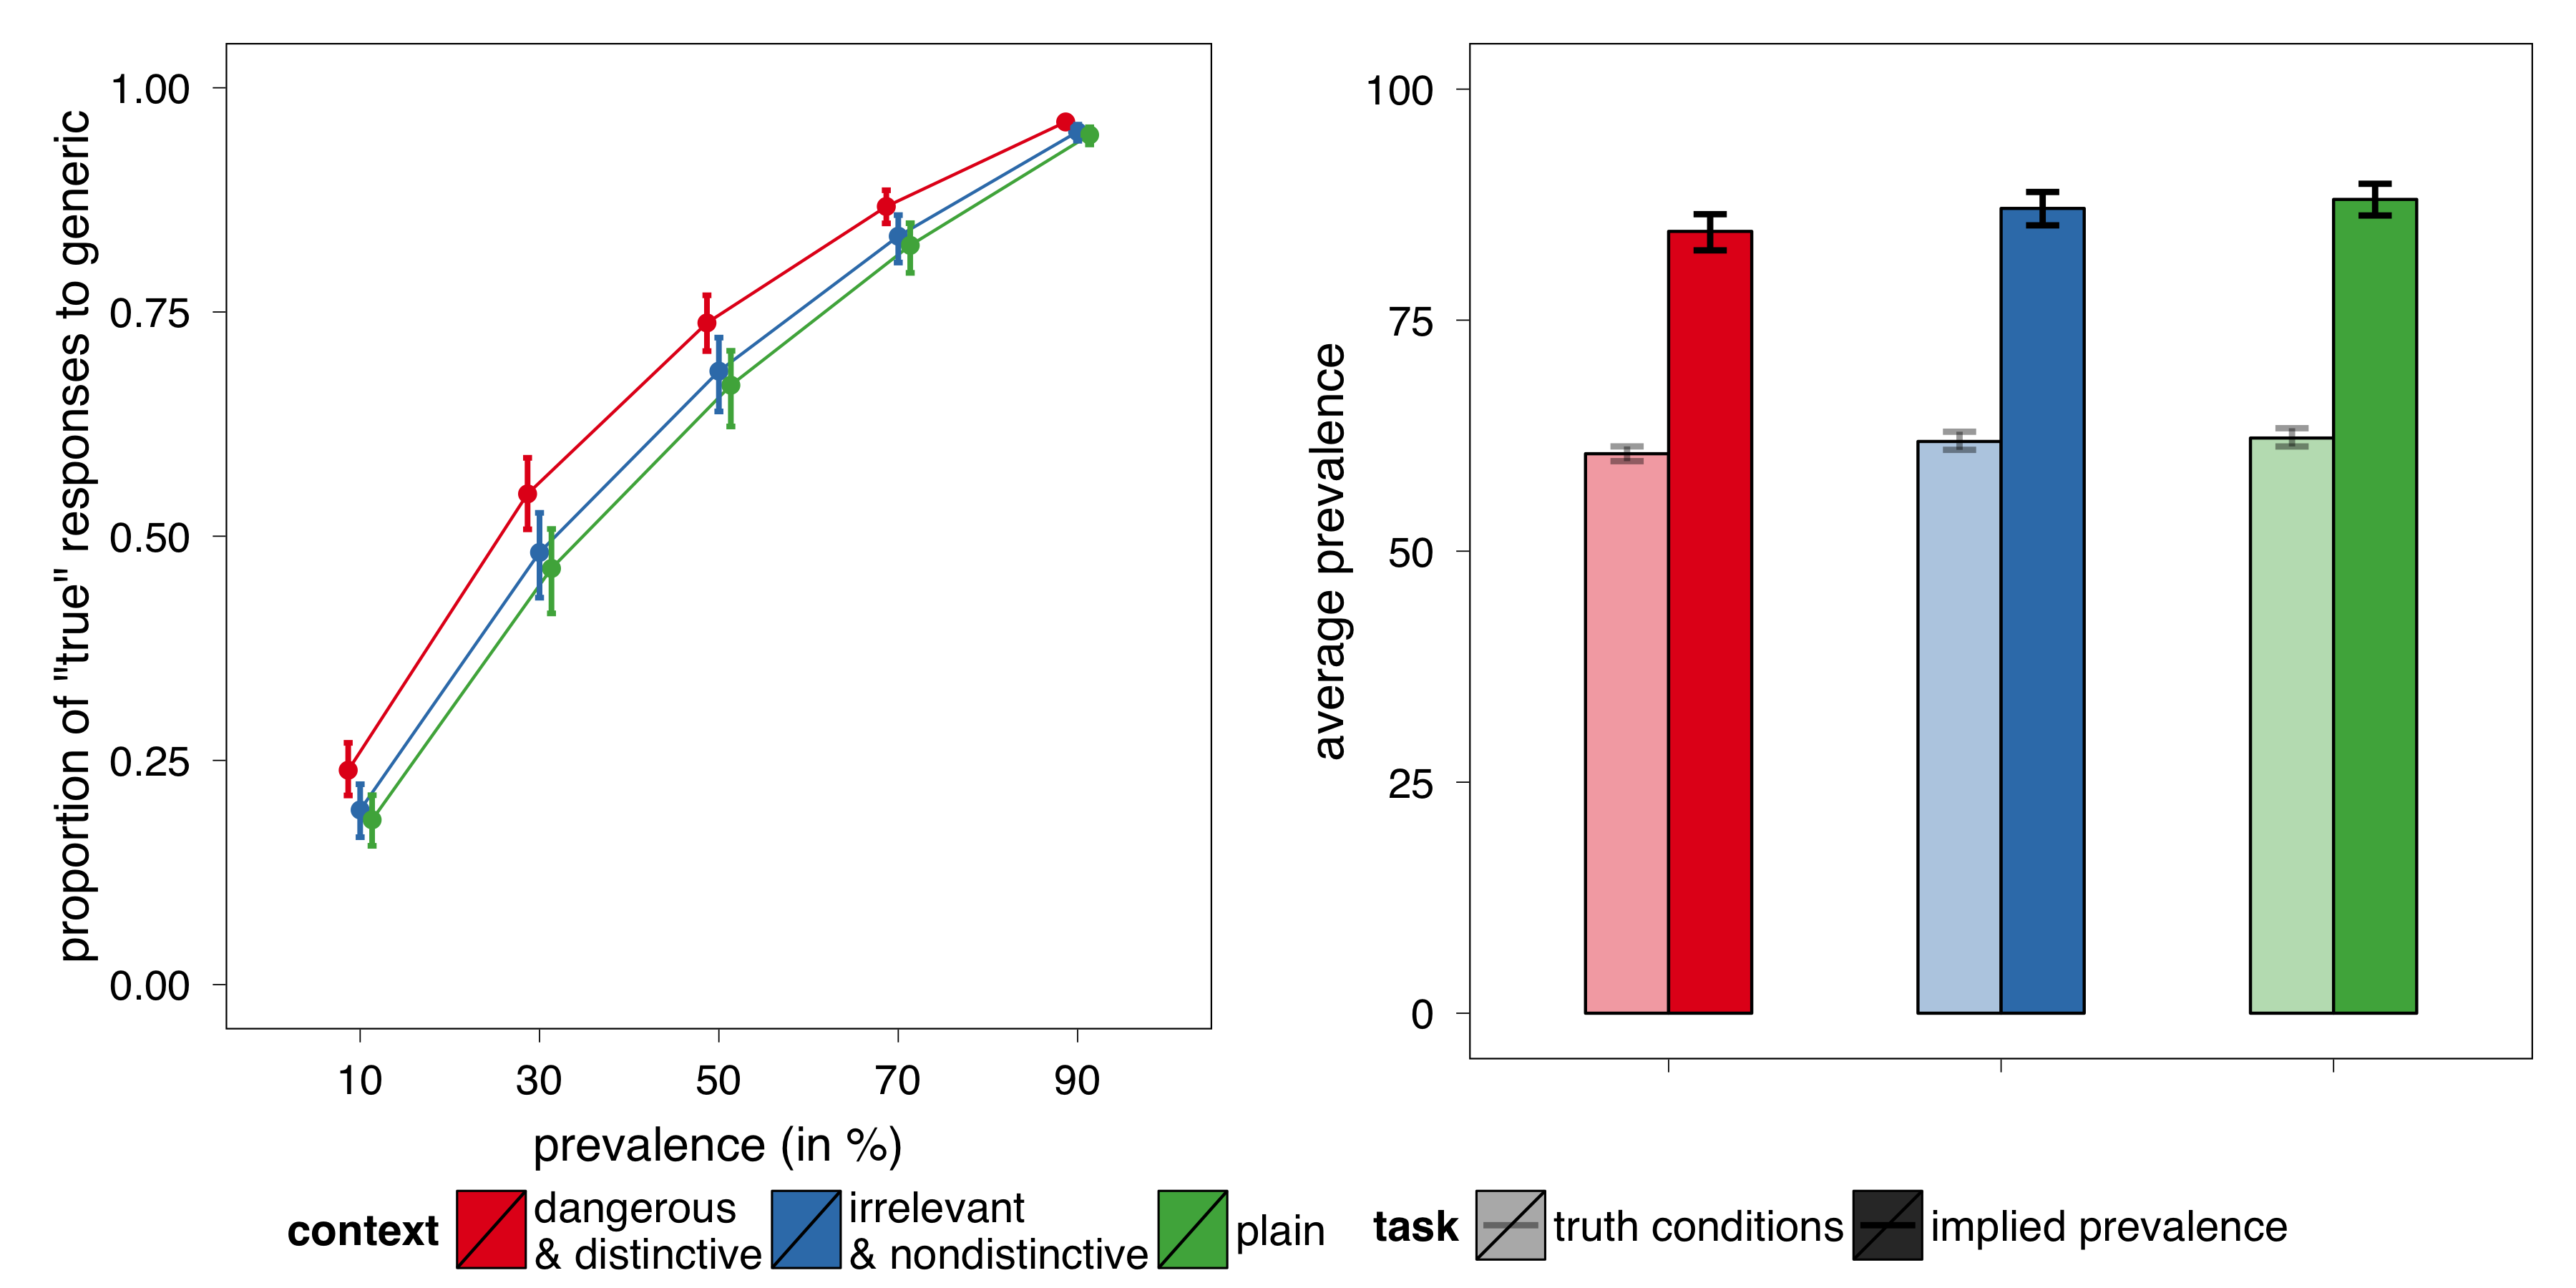
\includegraphics[width=\columnwidth]{lvRSA_postpreds}
    \caption{Posterior predictives of lifted-threshold RSA for truth conditions (left) and asymmetry between truth conditions and implications (right).}
  \label{fig:lvRSAposteriorpred}
\end{figure}

\subsection{Discussion}

To see how this asymmetry is possible, consider again the inferred prevalence priors in Figure \ref{fig:inferredpriors}. They are bimodal with peaks around 0\% and 100\%. This is consistent with the intuition that biological properties, such as the ones used by CBG, are properties either held by all of a category or none of a category. Since the semantics of the generic is underspecified (i.e. $\theta$---the threshold for truth judgement---is unknown), if $\theta$ falls anywhere in the range between 10\%-90\%, the most likely prevalence is going to be near 100\% (i.e. after ruling out 0\%, the next most-likely alternative is 100\%). Hence, in the \emph{implied prevalence task}, the most likely inferred prevalence could be appreciably higher than one would expect from the \emph{truth conditions} task. 




%\begin{figure}
%\centering
%    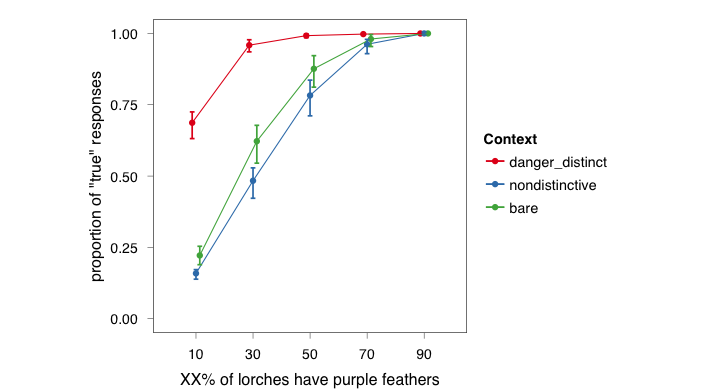
\includegraphics[width=\columnwidth]{fig5_bda2_postpred}
%    \caption{Posterior predictive using lifted-variable RSA}
%  \label{fig:postpred2}
%\end{figure}

Often in Bayesian data analysis, the posterior distribution over parameters is hard to interpret in terms of observable phenomena. Our case is not so opaque: if our model is the correct model of this task, the prior distributions of prevalence for the three property types should look like they do in Figure \ref{fig:inferredpriors}. 
In particular, all three types of properties should have bimodal prior prevalence distributions, with a high probability that 0\% of the kind have the property. Further, this left skew should be more pronounced for the \emph{dangerous and distinct} properties relative to the \emph{plain} properties. 

\section{Experiment 2}

\begin{figure}
        \centering
        \begin{subfigure}[b]{0.9\columnwidth}
    			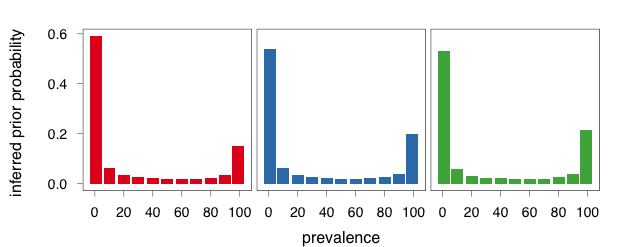
\includegraphics[width=0.9\columnwidth]{inferred_marginalized_priors1}
                \caption{Reconstructed priors from marginalized posterior $\gamma$ and $\delta$, for each property type.}
                \label{fig:inferredpriors}
        \end{subfigure}%
        
        %add desired spacing between images, e. g. ~, \quad, \qquad, \hfill etc.
          %(or a blank line to force the subfigure onto a new line)
        
        \begin{subfigure}[b]{0.9\columnwidth}
                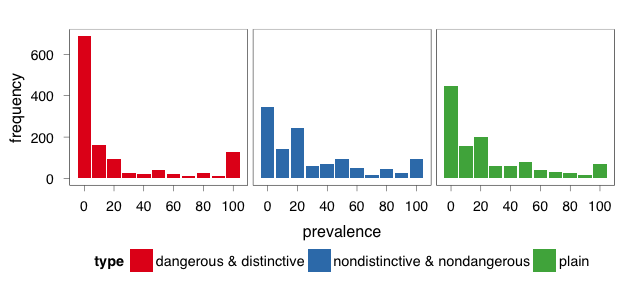
\includegraphics[width=0.9\columnwidth]{exp2_elicited_combined}
                \caption{Priors elicited in Experiment 2.}
                \label{fig:elicitedpriors}
        \end{subfigure}
        %add desired spacing between images, e. g. ~, \quad, \qquad, \hfill etc.
          %(or a blank line to force the subfigure onto a new line)
        \caption{Prior distributions over prevalence.}\label{fig:priors}
\end{figure}


%\begin{figure}
%        \centering
%        \begin{subfigure}[b]{\columnwidth}
%    			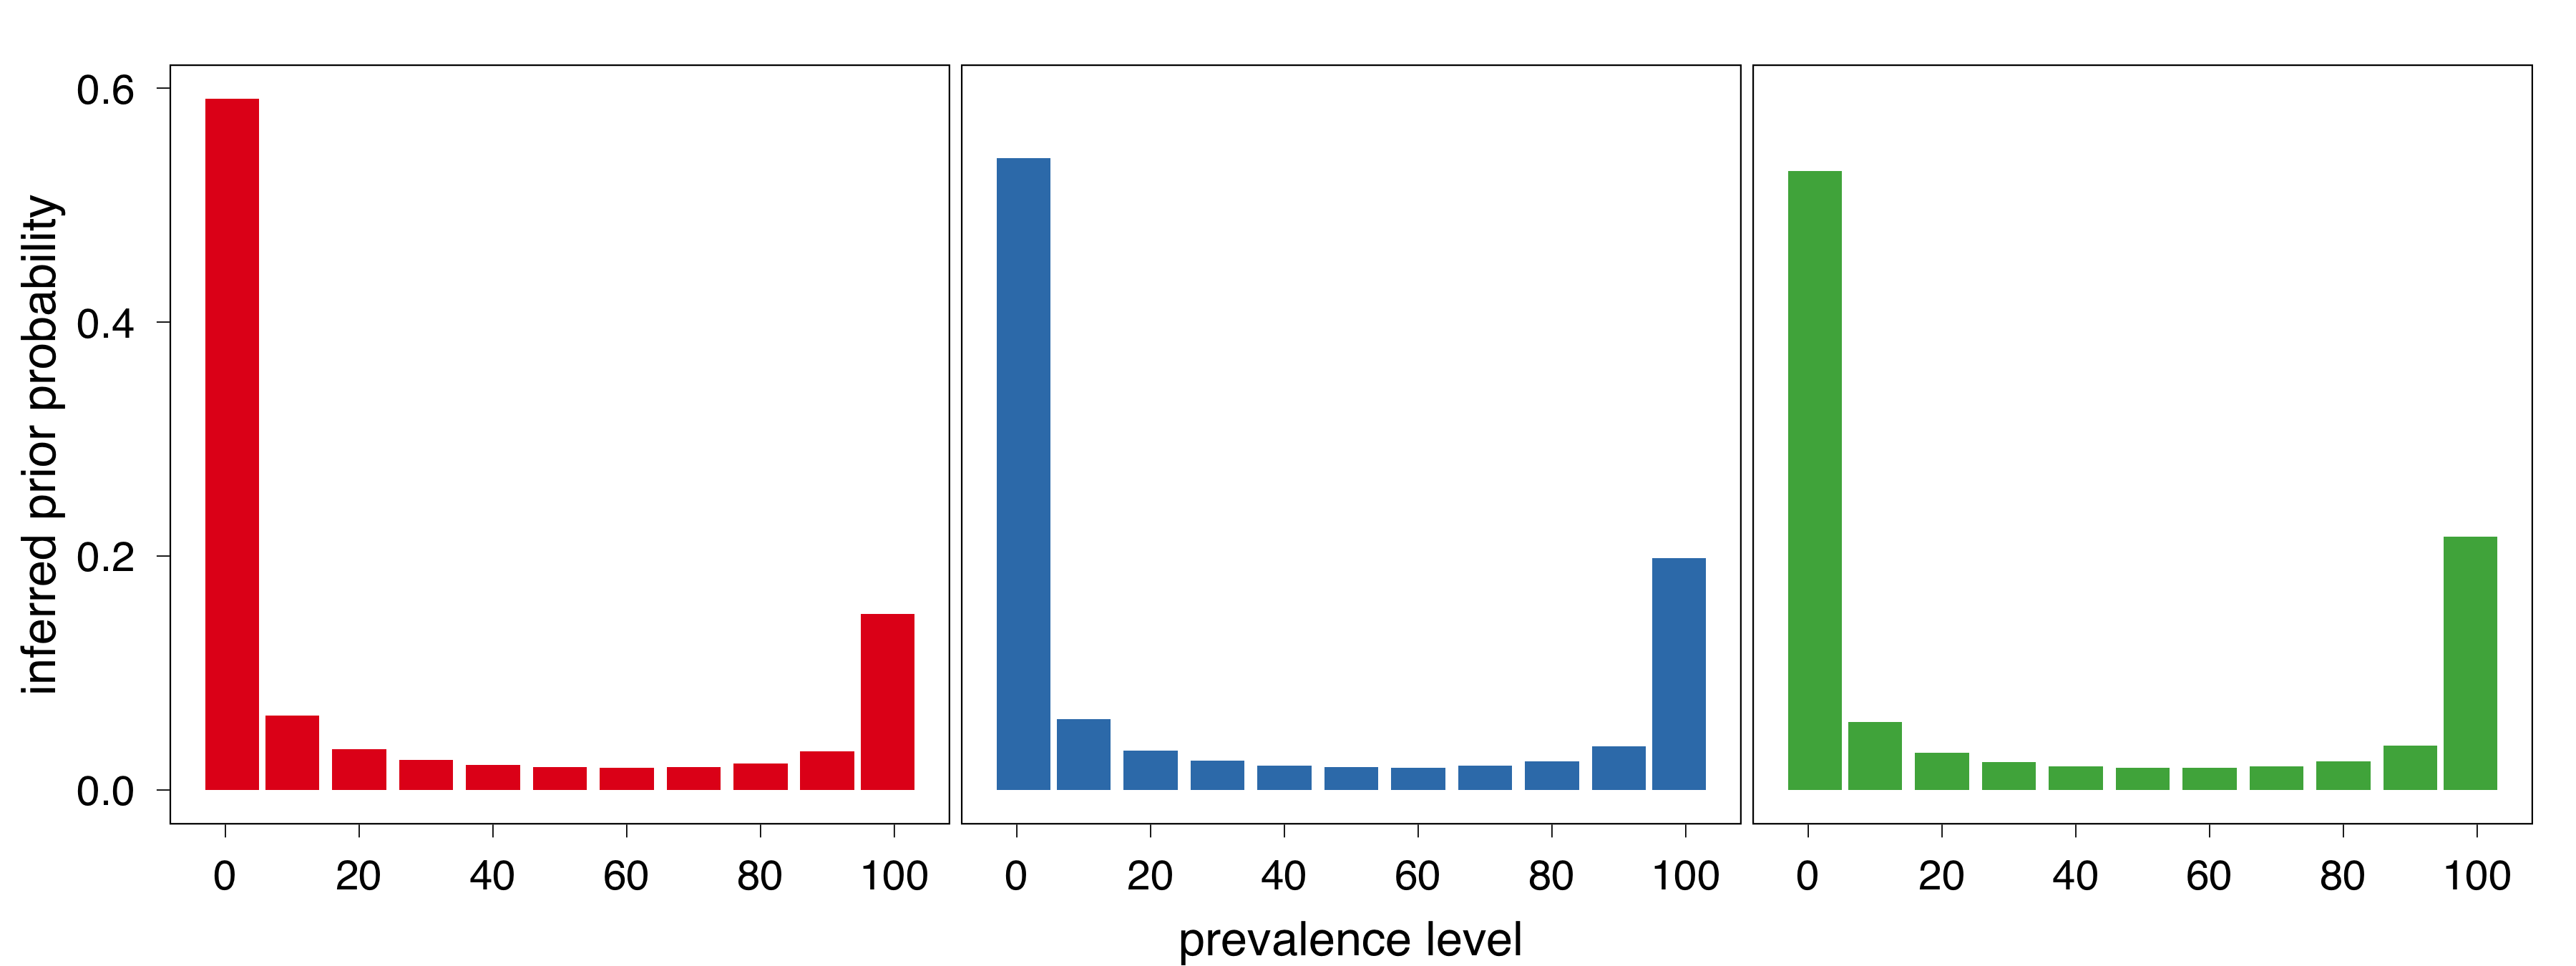
\includegraphics[width=\columnwidth]{inferred_marginalized_priors}
%                \caption{Reconstructed priors from marginalized posterior $\gamma$ and $\delta$, for each context.}
%                \label{fig:inferredpriors}
%        \end{subfigure}%
%        
%        %add desired spacing between images, e. g. ~, \quad, \qquad, \hfill etc.
%          %(or a blank line to force the subfigure onto a new line)
%        
%        \begin{subfigure}[b]{\columnwidth}
%                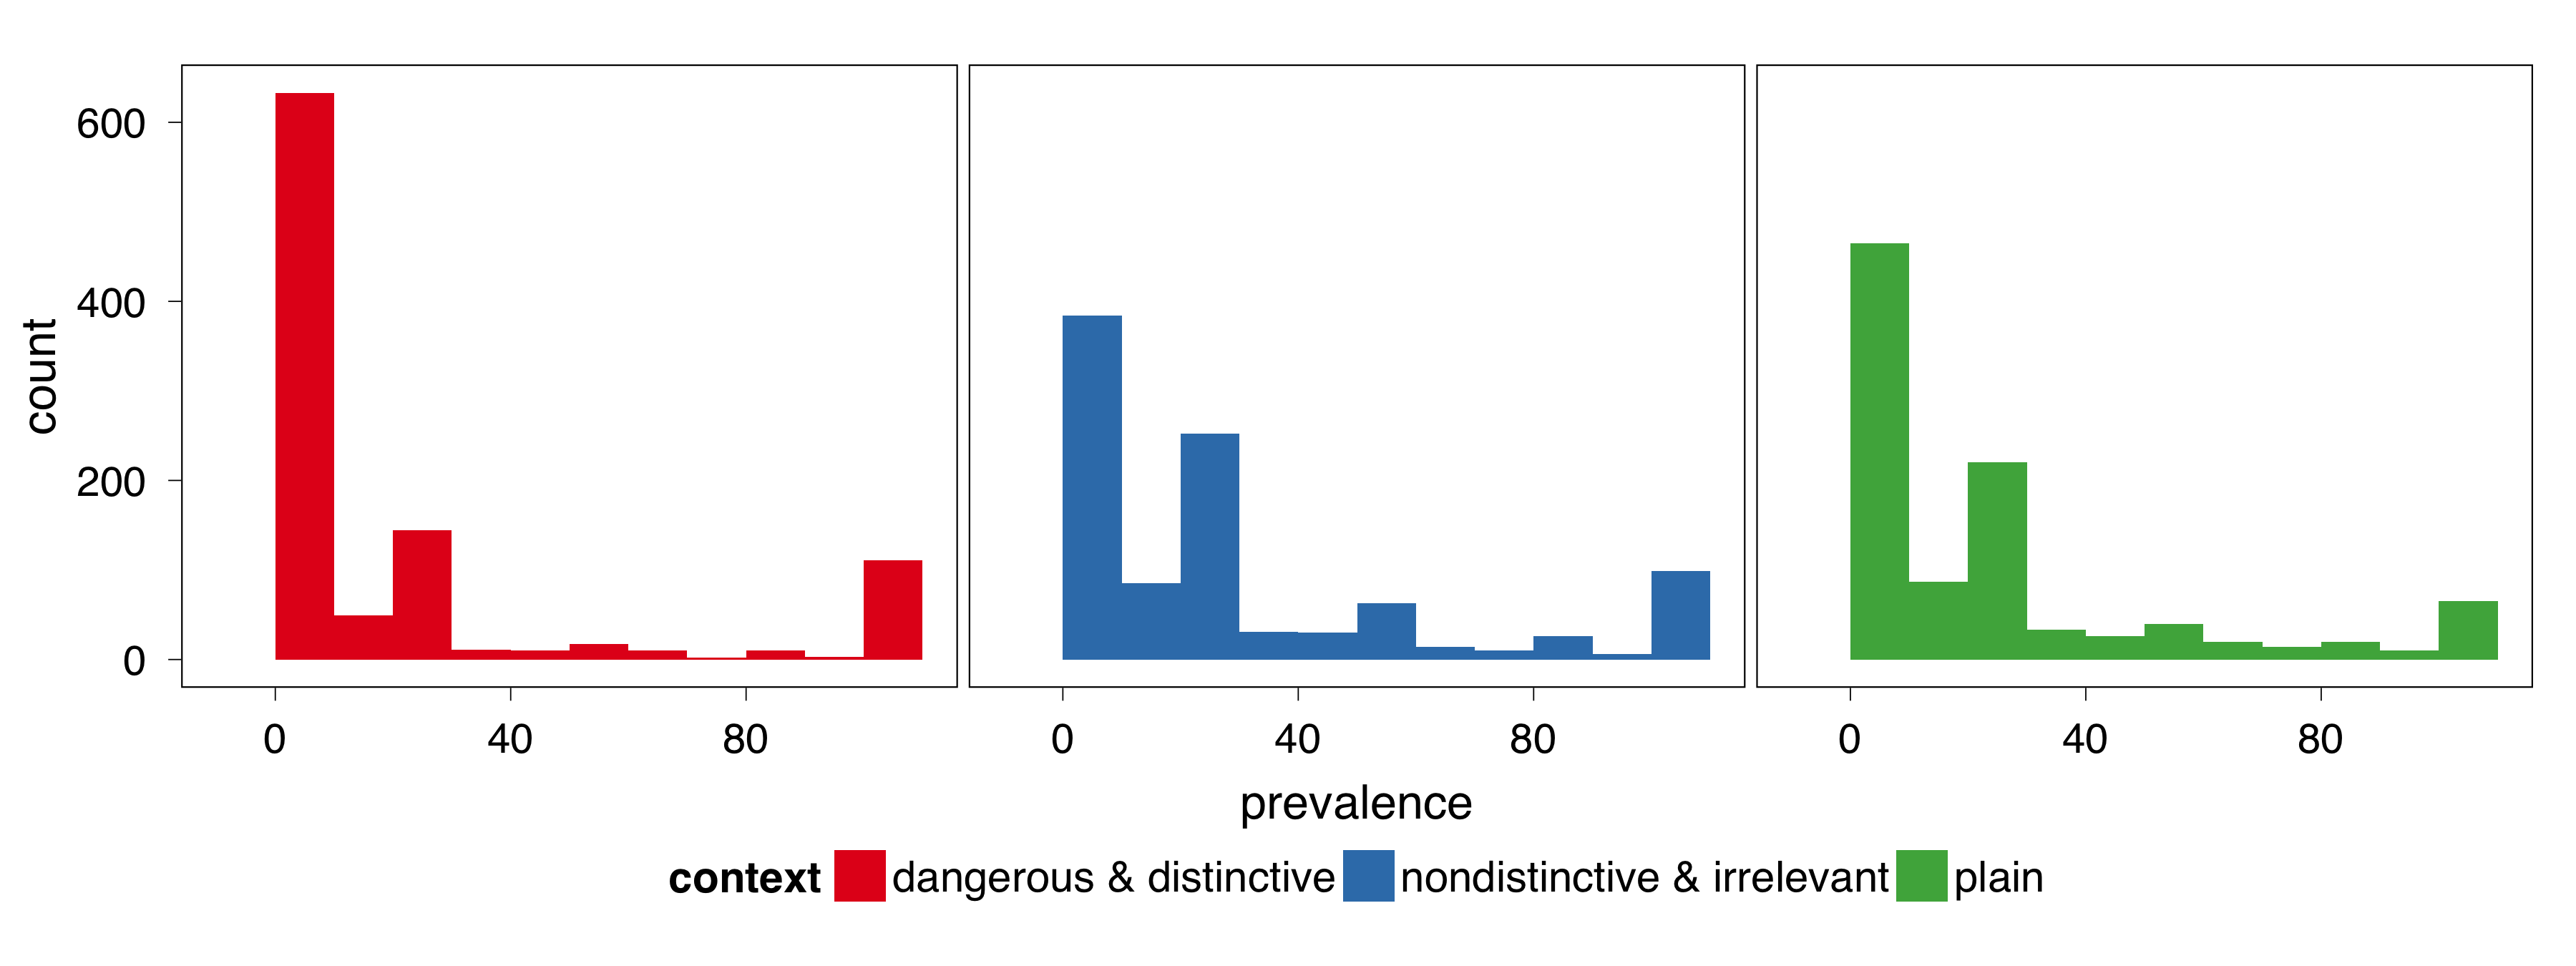
\includegraphics[width=\columnwidth]{elicited_priors}
%                \caption{Priors elicited in Experiment 2.}
%                \label{fig:elicitedpriors}
%        \end{subfigure}
%        %add desired spacing between images, e. g. ~, \quad, \qquad, \hfill etc.
%          %(or a blank line to force the subfigure onto a new line)
%        \caption{Prior distributions over prevalence.}\label{fig:priors}
%\end{figure}


Exp. 2 sought to test the prediction that the prior distribution of prevalence levels would be bimodal and vary by property type. The proper way to elicit prior beliefs about domains remains an open question in cognitive science. Here, we try 4 different dependent measures and assess their reliability with respect to each other.

\subsection{Method}

\subsubsection{Participants}

We recruited 120 participants over Amazon's crowd-sourcing platform Mechanical Turk. Participants were restricted to those with US IP addresses and with at least a 95\% MTurk work approval rating. All participants were native English speakers. The experiment took about 4 minutes and participants were compensated \$0.40.


\subsubsection{Procedure and materials}

Our procedure\footnote{The experiment in full can be viewed at \url{http://stanford.edu/~mtessler/experiments/generics/cbg2010-replication/experiment/experiment-11.html}} was similar to Exp. 1b. On each trial, participants either read information about the property type (\emph{dangerous and distinctive} or \emph{nondangerous and nondistinctive}) or nothing (\emph{plain}). 

In addition to the contextual information, participants were told: ``Listed below are X kinds of animals that are found on the island.'' and asked the following question: ``What percentage of each kind of animal do you think has [property]?'' 

Participants were either presented with 1, 5, or 10 animal-names per trials (between-subjects; ``Listed below is/are \{1, 5, 10\} kind(s) of animal(s) ...''). For these three groups (n=30 for each), the dependent measure was a free response (or 5 or 10) restricted to be a number between 0--100. A fourth group of participants (n=30) was run in just the 5 kinds/trial condition but with a dependent measure that was a slider bar that ranged from 0--100. The motivation for including multiple kinds per trial was to encourage participants to think about the \emph{distribution} of the property across animal kinds.

In total, participants gave 30 responses (equal numbers for each property type).

\subsection{Results}

The different dependent measures explored produced highly reliably results. QQ-plots revealed a strong linear relationship between the distributions of responses for each of 4 dependent measures used (95\% CI for average $r_{pearson} = [0.90,0.96]; r_{spearman}= [0.93,0.97]$). Hence, we collapsed across these dependent measures.

Experiment 2 recovered the shape of the inferred prior distributions predicted from the Bayesian analysis of the lifted-threshold RSA model (compare Figure \ref{fig:elicitedpriors} to Figure \ref{fig:inferredpriors}). 
%
Hartigans' Dip Test for Unimodality was highly significant for each of the prior distributions ($D = 0.054, 0.084, 0.0745$ for types \emph{dangerous and distinctive}, \emph{nondangerous and nondistinctive}, and \emph{plain}, respectively; p $<$ 0.0001 for each), and thus the distributions are at least bimodal. 
%
The means of these three distributions are distinct and ordered as predicted (bootstrapped 95\% confidence intervals in parentheses): $\mu_{dangerousdistinctive} = 18.1\% (16.0, 20.2), \mu_{plain} = 20.8\% (19.0, 22.5), \mu_{nondangerousnondistinctive} = 25.7\% (23.7, 27.6)$.
%
The medians of these three distributions were all significantly different from one another, evidenced by pair-wise Mann-Whitney U tests (\emph{dangerous and distinctive} vs. \emph{plain}: $W=417452$; \emph{dangerous and distinctive} vs. \emph{nondangerous and nondistinctive}: $W=376180.5$; \emph{nondangerous and nondistinctive} vs \emph{plain}: $W=548994.5$; all $p < 0.00001$). 
%
Finally, the distributions themselves were all significantly different from one another, by Kolmogorov-Smirnov tests (\emph{dangerous and distinctive} vs. \emph{plain}: $D = 0.185$;  \emph{dangerous and distinctive} vs. \emph{nondangerous and nondistinctive}: $D = 0.253$; \emph{nondangerous and nondistinctive} vs \emph{plain}: $D = 0.091$; all $p < 0.001$). In sum, the elicited prior distributions are all at least bimodal, have different central tendencies, and are all distinct in shape.


\subsection{Extension: Using the empirical priors}
\label{sec:emprior}

\begin{figure}
\centering
    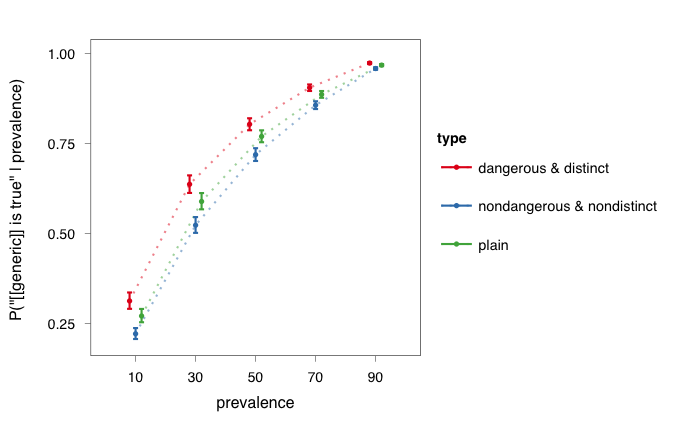
\includegraphics[width=\columnwidth]{exp1truthconds_empiricalPriors}
    \caption{``Forward'' predictions of lifted-threshold RSA for truth conditions using the empirical priors from Expt. 2.}
  \label{fig:exp1preds}
\end{figure}


In Section \ref{sec:model1}, we posited a family of priors for our model (the $\beta$ family of distributions). We saw that our model could accommodate both the flexibility in truth conditions as well as the asymmetry between truth conditions and implications. This combined data-analysis --- cognitive model made the \emph{backward prediction} that the priors would have to vary between property-types. In Exp.~2 we found that to be case \footnote{Qualitative differences between the \emph{observed} and \emph{backward-predicted} priors are likely a results of the family of priors posited a priori. The $\beta$ family can only accommodate U- and N- shaped distributions.}. There is still a question of whether or not the priors elicited in Exp.~2 would actually still predict the flexible truth conditions and the asymmetry.  

To test this, we fix the rationality parameters $\lambda_{task}$ as the fit-value to be the Maximum A-Posteriori (MAP) values from the Bayesian model analysis above. We then sample, with replacement, subjects from our prior elicitation task in order to bootstrap our model predictions. The confidence intervals thus reflect the uncertainty in our model predictions attributable to uncertainty in the empirical prior data\footnote{The model predictions are generated using exact enumeration, so there uncertainty in the model predictions due to posterior sampling error.}. 



Figure \ref{fig:exp1preds} shows the model predictions for the truth conditions using the empirical prior data from Expt. 2. Like the model with $\beta$ family hyperpriors, the empirical prior model captures the flexibility in truth conditions across the three property types. Figure \ref{fig:model_asyms} shows the predicted ``strong implications'' for the biological type properties used in Expt. 1.


\begin{figure}
\centering
    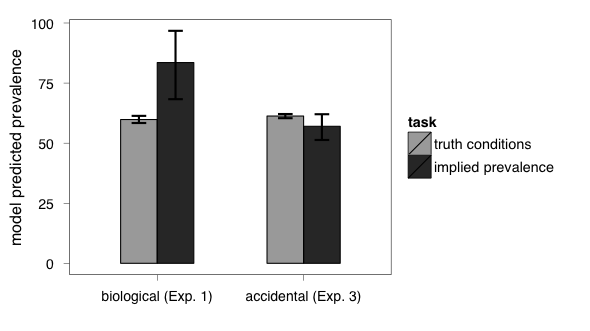
\includegraphics[width=0.8\columnwidth]{model_asymmetries}
    \caption{Lifted-threshold RSA coupled with empirical priors predicts strong implications for the ``biological'' properties used in Expt. 1, but not for the ``accidental'' properties used in Expt. 3.}
  \label{fig:model_asyms}
\end{figure}

We have seen thus far how a model that takes into account not only the prevalence of a particular property \emph{within} a category but also crucially \emph{across categories} can explain the flexibility in truth conditions of a number of different types of properties. We have also seen how bimodal ``biological'' priors can lead to near-universal implications for generic statements. In the experiments that follow, we explore cases where these effects break down.


\section{Experiment 3: Accidental properties}

The lifted-threshold model of generic meaning makes the further prediction that should the prior distribution over prevalence of the property \emph{not} have a peak at 100\%, the asymmetry should go away. That is, if the prior doesn't have a peak at 100\%, the \emph{implications} of a generic statement would not be as strong. CBG also made a similar prediction, though from a different theoretical perspective. They ran a version of the task using \emph{accidental} or \emph{temporary} states and found that the responses in the \emph{implied prevalence} task were significantly reduced (relative to the \emph{biological} type properties used in Exp.~1). In Experiment 3a, we sought to replicate this finding. In Experiment 3b, we measured the prior distribution over prevalence for these \emph{accidental} or \emph{temporary} properties.

\subsection{Experiment 3a: truth conditions and implications}

Experiment 3a differed from Exp.~1a \&b only in that there was only one property type: accidental or temporary properties. 

\subsubsection{Participants}

We recruited 100 participants over Amazon's crowd-sourcing platform Mechanical Turk. Participants were restricted to those with US IP addresses and with at least a 95\% MTurk work approval rating. All participants were native English speakers. The experiment took about 5 minutes and participants were compensated \$0.50.

\subsubsection{Procedure and materials}

Participants were randomly assigned to either the \emph{truth conditions} task (n=59) or the \emph{implied prevalence} task (n=41). Each task consisted of 20 items, all of which referred to temporary, accidental, or disease states (see CBG Appendix B for full list). In the truth conditions task, participants were given a prevalence statement (e.g. ``30\% of lorches have muddy feathers'') and asked if the corresponding generic statement (i.e. ``Lorches have muddy feathers'') was true or false. In the implied prevalence task, participants were given a given statement (e.g. ``Lorches have muddy feathers'') and asked to estimate the percentage of the kind that displayed that feature (i.e. what percentage of lorches have muddy feathers?)

\subsubsection{Results}

\begin{figure}
\centering
    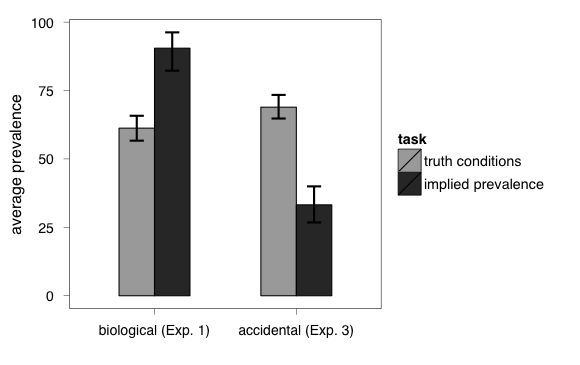
\includegraphics[width=0.8\columnwidth]{exp3_asymmetry}
    \caption{Implied prevalence of generic statements about biological (Exp.~1) and accidental (Exp.~3) are differentially associated with the truth conditions. Error bars denote bootstrapped 95\% confidence intervals.}
  \label{fig:exp3_asymm}
\end{figure}


We followed the data same data analysis strategy as in Exp.~1 and as in CBG. We replicate CBG's finding that the generic statement about accidental properties was not interpreted as applying to nearly all of the category. Figure \ref{fig:exp3_asymm} shows that difference between the two tasks, together with the data from Exp.~1, collapsed across property types (dangerous and distinct, etc...). \red{[Insert some boringly obvious statistics here.]}



\subsection{Experiment 3b}

Experiment 3b differed from Exp.~2 only in that there was only one property type: accidental or temporary properties. 

\subsubsection{Participants}

We recruited 40 participants over Amazon's crowd-sourcing platform Mechanical Turk. Participants were restricted to those with US IP addresses and with at least a 95\% MTurk work approval rating. All participants were native English speakers. The experiment took about 4 minutes and participants were compensated \$0.40.

\subsubsection{Procedure and materials}

Our procedure\footnote{The experiment in full can be viewed at \url{http://stanford.edu/~mtessler/experiments/generics/cbg2010-replication/experiment/prior-5.html}} was identical to Exp. 2. On each trial, participants were told: ``Listed below are 5 kinds of animals that are found on the island.'' and asked: ``What percentage of each kind of animal do you think has [accidental/temporary property]?'' 

In Exp.~2, we found high reliability between dependent measures in this prior elicitation paradigm. In this experiment, we ran only the condition with 5 animal-kinds per trial with a slider varying from 0--100 for each animal.


\subsubsection{Results}

% More active language; prior elictations

The elicited prior over prevalence for accidental properties was markedly different than the priors over the biological properties. Most importantly, there was no special status given to 100\% prevalence. \red{[What else to say about this...]}


\begin{figure}
\centering
    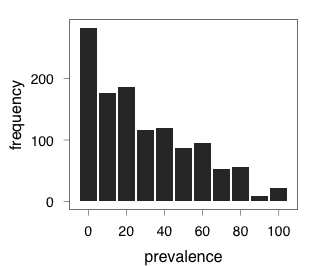
\includegraphics[width=0.5\columnwidth]{accidental_priors}
    \caption{Elicited prior distribution over prevalence of accidental properties.}
  \label{fig:accidentalpriors}
\end{figure}


\subsection{Modeling results}

We use the priors elicited in Exp.~3b to test if our model, like participants, infers a lower overall prevalence when interpreting a generic statement about accidental properties. Using the same bootstrapping method as describe in Section \ref{sec:emprior}, we generated model predictions for the truth conditions and implied prevalence tasks using the empirical priors elicited in Exp.~3b. Figure \ref{fig:model_asyms} (right) shows the predicted truth conditions and implications for generic statements about accidental properties. Like the human data, the model predictions much weaker implications for generics about accidental properties. This asymmetry goes away and begins to reverse.

Thus, we can see how the shape of the prior over prevalence is critical to fostering the strong implications of generic statements about biological properties. When properties with different shaped priors are under discussion (particularly, priors without large mass at 100\%), the asymmetry between truth conditions and implications can disappear or even reverse.

\section{Experiments 4: Dangerous properties}

Our model explains the flexibility of truth conditions in terms of the prior distribution over prevalence. One potential challenge to this is that properties which are not necessarily \emph{distinctive} still garner acceptability as generic statements. For example, CBG found that \emph{dangerous} properties alone increased the proportion of ``true'' responses to the generic. Here, we sought to replicate these findings, and observe if the prior distribution over \emph{dangerous} properties was in fact similar to the prior distribution over \emph{distinctive} properties. That is, are \emph{dangerous} generics endorsed by virtue of the fact that dangerous properties are distinctive properties?

\subsection{Experiment 4a: truth conditions}

Experiment 4a differed from Exp.~1a only in that the three property types tested were \emph{dangerous} (e.g. ``These feathers are as sharp as needles and can easily get lodged in you, causing massive bleeding''),  \emph{distinctive} (e.g. ``No other animals have these kinds of feathers''), and \emph{plain} (no additional information). 

\subsubsection{Participants}

We recruited 80 participants over Amazon's crowd-sourcing platform Mechanical Turk. Participants were restricted to those with US IP addresses and with at least a 95\% MTurk work approval rating. All participants were native English speakers. The experiment took about 5 minutes and participants were compensated \$0.50.

\subsubsection{Procedure and materials}

All participants were assigned to the \emph{truth conditions} task \footnote{The experiment in full can be viewed at \url{http://stanford.edu/~mtessler/experiments/generics/cbg2010-replication/experiment/experiment-15.html}}. 
 
We used the same materials as CBG (available in their Appendix). The materials used were 30 novel animal categories (e.g. lorches, morseths, blins) each paired with a unique property. Properties were made by pairing a color with a body-part (e.g. purple feathers, orange tails). Each participant saw 30 unique animal-property pairs: 10 of each of the 3 types (\emph{dangerous}, \emph{distinctive}, \emph{plain}). The 10 items of each property-type were randomly paired with 1 of 5 ``prevalence levels'': \{10, 30, 50, 70, 90\}\%; thus, each prevalence level appeared 2 times per type. 

On each trial, participants saw a prevalence statement and type statements (\emph{dangerous}, \emph{distinctive}, \emph{plain}; illustrated above). 
%A context here was either (1) dangerous \& distinct statements (e.g. ``These feathers are as sharp as needles and can easily get lodged in you, causing massive bleeding. No other animals have these kinds of feathers.''), (2) not distinct \& irrelevant statements (e.g. ``These feathers are wide and very smooth to the touch. Other animals have these kinds of feathers.'', or (3) nothing else. 
Participants were then asked ``Is the following sentence true or false?'', below which was presented the associated generic (e.g. ``Lorches have purple feathers'') and ``True'' and ``False'' radio buttons. 
 
\subsubsection{Results}

\begin{figure}
\centering
    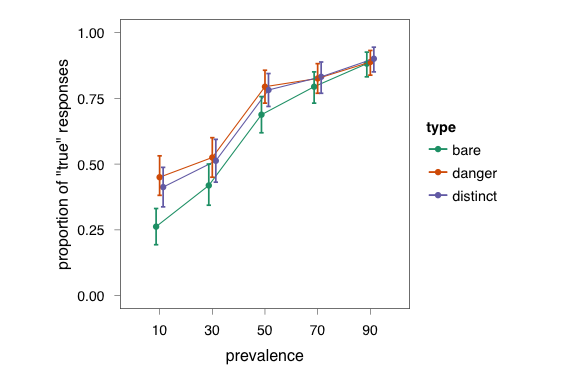
\includegraphics[width=0.8\columnwidth]{dd_separate_truthconds}
    \caption{Replication of CBG Exp. 4. Truth conditions for dangerous and distinctive properties (separately) are more relaxed than for plain properties.}
  \label{fig:ddseparate}
\end{figure}

Results are shown in Figure~\ref{fig:ddseparate}. We entered participants' truth judgments into a mixed effects logistic regression with random by-item and by-participant effects of intercept and fixed effects of prevalence and type as well as their interaction\footnote{This was the maximal mixed-effect structure supported by the data.}.  
%
Our results replicated the finding of CBG that the generic statements were endorsed more with dangerous properties and with distinctive properties than with plain properties ($\beta_{danger}=0.85; SE = .18; z = 4.69; p < .001; \beta_{distinct}=0.83; SE = .18; z = 4.53; p < .001$). 
%
There was also an interaction between prevalence level and type such that the generic was endorsed more with \emph{dangerous} properties than with plain properties at lower prevalence levels ($\beta=.02; SE = .007; z=2.76; p < 0.01$). There was a trending interactive effect for the \emph{distinctive} properties to be endorsed \emph{more} than the plain properties at low prevalence levels ($\beta=.01; SE = .007; z=1.67; p < .1$).


\subsection{Experiment 4b: prior elicitation}

Experiment 4b differed from Expt.~2 only in that the the dangerous and distinctive category was broken up into two categories (\emph{dangerous} and \emph{distinctive}, separately). The only other category tested were ``plain'' properties (no additional information provided).

\subsubsection{Participants}

We recruited 100 participants over Amazon's crowd-sourcing platform Mechanical Turk. Participants were restricted to those with US IP addresses and with at least a 95\% MTurk work approval rating. All participants were native English speakers. The experiment took about 4 minutes and participants were compensated \$0.40.

\subsubsection{Procedure and materials}

Our procedure\footnote{The experiment in full can be viewed at \url{http://stanford.edu/~mtessler/experiments/generics/cbg2010-replication/experiment/prior-5.html}} was identical to Exp. 2. On each trial, participants either read information about the property type (\emph{dangerous} or \emph{distinctive}) or no additional information (\emph{plain}). 

In addition to the information about property type, participants were told: ``Listed below are 10 kinds of animals that are found on the island.'' and asked: ``What percentage of each kind of animal do you think has [property]?'' In Exp.~2, we found high reliability between dependent measures in this prior elicitation paradigm. In this experiment, we ran only the condition with 10 animal-kinds per trial with a free response restricted to be a number between 0--100 for each animal.

\subsubsection{Results}

\begin{figure}
\centering
    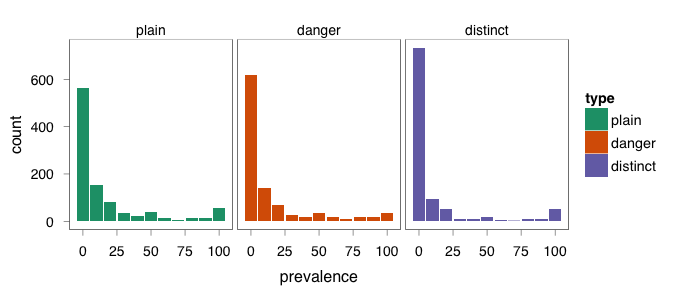
\includegraphics[width=0.8\columnwidth]{prior_ddp}
    \caption{Elicited prior distribution over plain, dangerous, and distinctive properties.}
  \label{fig:empiricalddp}
\end{figure}


Experiment 4b recovered the shape of biological property prevalence distributions (Figure \ref{fig:empiricalddp}). 
%
Hartigans' Dip Test for Unimodality was highly significant for each of the prior distributions ($D = 0.062, 0.039, 0.054$ for types \emph{plain}, \emph{dangerous}, and \emph{distinctive}, respectively; p $<$ 0.0001 for each), and thus the distributions are at least bimodal. 
%
The means of these three distributions are distinct and ordered (bootstrapped 95\% confidence intervals in parentheses): $\mu_{plain} = 16.6\% (14.9, 18.3), \mu_{dangerous} = 14.3\% (12.8, 16.0), \mu_{distinctive} = 11.1\% (12.7, 9.5)$.
%
The medians of these three distributions were all significantly different from one another, evidenced by pair-wise Mann-Whitney U tests (\emph{dangerous} vs. \emph{plain}: $W=527732.5$; \emph{distinctive} vs. \emph{plain}: $W=596451.5$; \emph{distinctive} vs \emph{dangerous}: $W=570639.5$; all $p < 0.05$). 
%
Finally, the distributions themselves were all significantly different from one another, by Kolmogorov-Smirnov tests (\emph{dangerous} vs. \emph{plain}: $D = 0.062$;  \emph{dangerous} vs. \emph{distinctive}: $D = 0.142$; \emph{distinct} vs \emph{plain}: $D = 0.197$; all $p < 0.05$). In sum, the elicited prior distributions are all at least bimodal, have different central tendencies, and are all distinct in shape.


\subsection{Modeling results}

We followed the same model analysis as in Section \ref{sec:emprior}. We bootstrapped the model predictions by resampling (with replacement) the empirical prior judgments of Expt. 4b. The model predictions for the truth conditions of separate dangerous and distinct (as well as plain) properties are shown in Figure \ref{fig:tcddb}. The model predicts an overall higher proportion of ``true'' responses to the generic at low prevalence levels for \emph{distinctive} properties relative to \emph{plain} properties. It is unclear whether or not the model also predicts a reliable overall higher proportion of ``true'' responses at low prevalence levels for \emph{dangerous} properties relative to \emph{plain} properties. 

\begin{figure}
\centering
    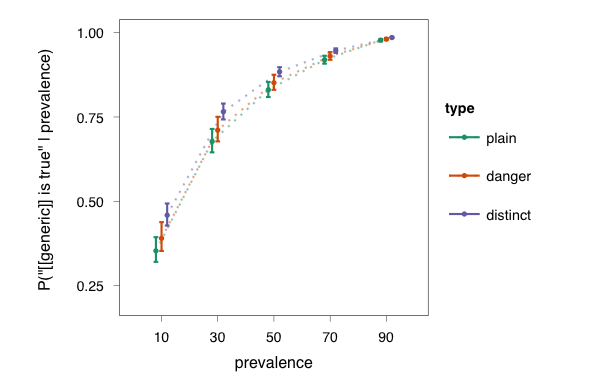
\includegraphics[width=0.8\columnwidth]{ddb_bootstrap_truthconds}
    \caption{Model predictions for truth conditions of dangerous, distinctive, and plain properties. Error bars denote bootstrapped 95\% confidence intervals.}
  \label{fig:tcddb}
\end{figure}


\section{General discussion}

The lifted-threshold RSA model presented in this paper takes a generic statement to be vague. ``X has Y'' means ``many X have Y, \emph{relative to other categories, the vast majority of which, very few or none of the individuals in those categories have Y}''. The model predicts overall more relaxed truth conditions for generics of properties that have prevalence distributions which place significant probability mass at or near 0\% and significant probability mass at some prevalence greater than 0\%. By reasoning pragmatically about an uncertain threshold, the model is able to arrive at gradable and context-sensitive predictions about the truth conditions and implications of generic statements. 

We used a Bayesian data analytic model to make a ``backward prediction'' about the underlying prevalence prior by way of the observed experimental generics data and the lifted-threshold RSA model. We verified this prediction and then incorporated the empirical prior into the model, reconfirming the original fit. We showed how our model predicts a dissipation (or even reversal) of the asymmetry between truth conditions and implications of generics as first explored by \citeA{Cimpian2010}. Finally, we explored how far prevalence alone could take us, by measuring the prior for just \emph{dangerous} properties. We found that while \emph{dangerous} properties were interpreted as more distinctive and plain properties, this difference only led to marginal increases in the predicted ``true'' responses in the truth conditions task. 

The observation that the predictions for the truth conditions task were \emph{qualitatively} correct but \emph{quantitatively} not as large as the observed behavior data gives rise to at least two possible explanations. First, it is possible that our technique for measuring the prior distribution over prevalence is too crude to account for such small differences in prevalence. It was not guaranteed that differences in the truth conditions tasks between truth judgments at different prevalence levels would actually show up as important differences in the prior elicitation task. 
Additionally, the measurements made in the truth conditions task might also be too coarse: In these experiments, truth conditions are measured by categorical judgments (\emph{true} or \emph{false}) at prevalence intervals of 20\%. It's possible that more graded judgments at finer prevalence scales would be helpful in mediating this. However, it's also possible that with an uncertain threshold for the generics, participants will adapt to whatever prevalence sampling an experimenter presents. At the end of the day, the truth conditions task is interested in measuring the prevalence level at which the generic is true. It's likely that other, convergent measures would be helpful in assessing this. 

A second possibility for the seeming failure to account for the magnitude of the effect in truth judgments for different property types is because prevalence alone is not being used as the only measuring stick for assessing the generic. It's possible that something about the salience of the property (e.g. instantiated in its dangerousness) leads ones to be more flexible in its usage\cite{Leslie2008}. This explanation could be cashed out in a model of nonliteral language like the one in presented by \citeA{Kao2014}. The idea here would be that using a generic to describe a salient (e.g. dangerous) property of a kind would be like using hyperbolic language. This type of generic, then, would convey the idea of prevalence in addition to an affective message, like ``be careful''. We leave for future work exploring this type of explanation in more detail.


\subsection{The parallel problem of generic identification}

In this article, we have focused exclusively on the problem of generic meaning, using sentences with bare plural construction. The bare plural construction is likely the easiest for generic readings. For example, in the work of \citeA{Prasada2013}, the overall ``true'' responses for statements in the bare plural construction (regardless of content) was appreciably higher than all other sorts of constructions associated with generic meaning. In a way, bare plurals are only read generically. 

Stepping outside of bare plurals, one runs into a problem parallel to that of generic meaning: generic identification. There is no `generic operator' that signifies a particular sentence is a generic. Sentences of the same morphosyntactic type can take both generic and non-generic readings. For example, ``The bird is in the garage'' cannot be read generically while ``The bird is a warm-blooded animal'' can. Sensitivity to contextual and morphosyntactic cues begins early on \cite{Cimpian2008}. It's agreed that world-knowledge must exert influence at some level, e.g. to understand the different readings in ``A horse is sick'' vs. ``A horse is vegetarian'' \cite{Gelman2004}. It's likely the sort of knowledge used in the lifted-threshold RSA model (i.e. knowledge about the distribution of prevalence) would be useful in the problem of generic identification. 

\subsection{Generics in learning}

In this work, we have found that differences in the distributions of prevalence can explain differences in truth conditions for different types of properties. An open question for this line of work is how do children come to have different priors for different property types in the first place? It's estimated that generics account for 4\% of all utterances addressed to preschool-age children in everyday contexts \cite{Gelman2008} and that 2-3 year old children comprehend generic statements \cite{Cimpian2011, Gelman2003}. If interpreting a generic requires knowledge about the distribution of the prevalence of the property, where do children learn that from? One answer might be that learn it at the same time that they learn the meaning of the word in the first place \cite{Frank2009}. Further work should explore the learning problem in terms of a joint inference about the possible category in reference and the still-being-learned meaning of words. 
 
\subsection{Conclusion} 


We have explored and demonstrated the viability of a scalar semantics for generics when coupled with a sophisticated pragmatics. 
A lower-bound threshold on prevalence---the probability of the property given the category---is inferred as part of pragmatic interpretation, yielding vague and context sensitive meanings. 
%We first used Bayesian data analysis to show that the effective threshold of a fixed-threshold semantics would need to vary by context, and yet it still not account adequately for the data. 
%
%
We formalized reasoning about the threshold in a lifted-threshold Rational Speech Acts model. This model predicted graded truth judgements and an asymmetry between truth and prevalence judgments. It also naturally accommodates the role of context, explaining these effects as the result of variation in the prevalence prior. 

Generics are ubiquitous in natural language. It might seem paradoxical, then, that the semantics of generic statements are underspecified. Why should vague language get so much usage? One possibility is apparent in the lifted-variable RSA model: generic language provides interlocutors with the flexibility to convey rich meanings, which are easily understood in context. 
Generics are vague, but predictable and useful.


%In Experiment 2, we verified that participants' beliefs about the prior on prevalence varied in this way. 
%This provides evidence that the model we propose can account for many of the empirical phenomena associated with generics.

%We have shown how a Bayesian model of language understanding, motivated by contextual variation of the effective threshold of the generic statement, can explain the puzzling truth conditions and asymmetrical meanings of generic language. We have used techniques in Bayesian data analysis to help arbitrate between two cognitive theories. The first was a simple theory that proposed that a generic was akin to some alien quantifier. In this theory, the generic behaves like other quantifiers in that it has a fixed-threshold semantics. We explored one elaboration of this in allowing the generic to have a threshold that differed across contexts. 
%
%The alternative theory is that there is no generic threshold out there in the world to observe. Instead, listeners infer the threshold (and thus, the semantic content) of the words from context. The posterior predictive distributions of the lvRSA model account for the contextual variation in the generic endorsements, both quantitatively and qualitiative. It further accounts for the asymmetry between verification and interpretation by considering different Questions Under Discussion (QUDs) and communicative roles (speaker / listener) in the two tasks. Finally, the Bayesian analytic techniques allowed us to make a new prediction as to the shape of the prior distribution over prevalence levels for different contexts. Exp. 2 found confirmatory evidence that this is indeed how people think these properties are distributed.

%\section{Further simulations}
%
%Our model makes the prediction that if the shape of the prior distribution was not bimodal, the asymmetry between verification and interpretation would change. Indeed, this is a similar prediction to \citeA{Cimpian2010}, who posited that accidental or disease states (e.g. ``muddy feathers'', ``infected ears'') would weaken the asymmetry. We would expect accidental or disease states to not follow a bimodal distribution. 
 




%\begin{itemize}
%
%\item Replace figure 4 (hyperprior parameters) with mean distribution?
%
%\item Collapse Figure 3 \& 5 (posterior predictive) into one
%
%\item Exp 2 to confirm $\gamma$ and $\delta$. 
%
%\item Some linking function to condition on Exp 1 \& 2 simultaneously,  to perhaps, infer rationality parameter and get some posterior predictives.
%
%\end{itemize}
%
%The data analysis involved comparing the mean of the prevalence ratings associated with \emph{True} endorsements of the generic with the mean prevalence ratings elicited by the generic in a separate task. In the experimental pragmatics literature, the dependent measure involved in the ``truth conditions'' task is called \emph{sentence verification}; in the ``implied prevalence'' task, it is a \emph{sentence interpretation}. 
%
%These different dependent measures, we argue, imply different Questions Under Discussion (QUD, \cite{Roberts2004}). 



%	\section{Sentence verification is a speaker task}
%	
%	DegenGoodman2014.  Truth conditions task --> QUD = ``generic true?'' Model.
%	
%	But what is the semantics of the generic? \citeA{Cimpian2010}, experiments 1, 3, and 4 found that the truth conditions of the generic are sensitive to the context.  Our goal is to replicate this finding, and use Bayesian data analysis to infer the threshold of the speaker model. This bears some similarity to Michael Franke's approach for cogsci from last year.
%	
%	
%	
%	
%	\section{The full bayesian thing}
%	
%	Computational models of cognition typically have parameters. Many of these parameters are of theoretically interest, because they are posited to reside within the head of the subject.
%	
%	\subsection{Inferring quantifier threshold by context}
%	
%	Here we'll find that the generic threshold changes by context. We might also want to show that ``most'' and ``some'' do not change by context.
%	
%	\subsection{Are generics like adjectives?}
%	
%	To determine if a generic is true or false, we must refer to context. The threshold in the threshold-semantic view of the statement varies by context. This property has been shown to be an important feature in the semantics of gradable adjectives (e.g. \emph{tall}) \cite{Lassiter2014}.  
%	
%	\section{Lifted-variable speech act model}
%	
%	We can start in a single context, with a uniform prior over states. We can look at the posterior over states, for listener1. As well, we can look at the posterior over thetas. This depends of course on the alternatives, for which we may want to consider only the experimental alternatives \emph{some, most, generic} or for which we may want to include \emph{all}.  Either way, here we'll recreate the asymmetry between listener and speaker --- between implied prevalence and truth conditions. 
%	
%	\citeA{Cimpian2010} report a ``paradoxical asymmetry at the core of generic meaning'' which manifests as the generic having ``extremely strong implications but requiring little evidence to be judged true''. Here, we explain this ``paradox'' by the different Questions Under Discussions in the tasks used and by the different roles intrinsic to speech-acts: the role of the speaker and the role of the listener. 
%	
%	\subsection{Questions Under Discussion in two tasks}
%	
%	\citeA{Cimpian2010} used two tasks (with different dependent measures) to get at the comparison between ``acceptance'' and ``implications''. These two tasks --- called ``truth conditions'' and ``implied prevalence'' -- used different questions and different dependent measures to get at the meaning of generics. In the ``truth conditions'' task, subjects are given evidence about the prevalence of a property (e.g. ``50\% of morseths have silver fur'') and are asked to judge the corresponding generic (i.e. ``Morseths have silver fur'') to be either true or false. In the ``implied prevalence'' task, subjects are given a generic statement and asked ``What percentage of morseths do you think have silver fur?''
%	
%	\citeA{Degen2014} argue that the \emph{sentence verification} (``truth conditions'') task should be modeled as a speaker task, and that the \emph{sentence interpretation} (``implied prevalence'') task should be modeled as a listener task. In addition to different communicative roles, there are also different implicit Questions Under Discusision. In the ``truth conditions'' task, the QUD seems to be ``is the generic true or false?'', whereas in the ``implied prevalence'' task, the QUD seems to be ``what percentage of category X have property Y?''.





\bibliographystyle{apacite}

\setlength{\bibleftmargin}{.125in}
\setlength{\bibindent}{-\bibleftmargin}

\bibliography{generics}


\end{document}


% after cogsci
% prior elicitation for accidental / disease states
% -- asymmetry weakened

% most / some: better experiments
% -- asymmetry X prior analysis

